% !TEX program = pdflatex
% !TEX root = Bernal_H.tex
% !TEX outputDirectory = out
% Econometrica initial submission (ecta_template.tex / ecta_sample.tex)
% English version translated from Identification_of_rational_types_esp.tex
% Submit as a single .tex file with [draft] for initial submission.
\documentclass[ecta,nameyear,draft]{econsocart}

\RequirePackage[colorlinks,citecolor=blue,linkcolor=blue,urlcolor=blue,pagebackref]{hyperref}
\RequirePackage{float}
\RequirePackage{graphicx}
\RequirePackage{subcaption}
\captionsetup[figure]{skip=2pt}
\captionsetup[subfigure]{skip=1pt,font=footnotesize}
\setlength{\abovecaptionskip}{2pt}
\setlength{\belowcaptionskip}{0pt}
\setlength{\intextsep}{4pt plus 1pt minus 1pt}
\setlength{\textfloatsep}{6pt plus 2pt minus 2pt}
\setlength{\floatsep}{3pt plus 1pt minus 1pt}
\newlength{\subfigheight}
\setlength{\subfigheight}{4.2cm}
\newlength{\mapfigheight}
\setlength{\mapfigheight}{4.55cm}
\newlength{\widefigheight}
\setlength{\widefigheight}{3.4cm}
\newlength{\calfigheight}
\setlength{\calfigheight}{3.2cm}
\newlength{\calbeliefheight}
\setlength{\calbeliefheight}{4.5cm}
\newlength{\calseriesheight}
\setlength{\calseriesheight}{3.8cm}
\newlength{\calplotheight}
\setlength{\calplotheight}{4.2cm}
\newlength{\calpathheight}
\setlength{\calpathheight}{5.1cm}
\newcommand{\panelgraphic}[2]{%
  \parbox[t][#1][t]{\linewidth}{\centering\includegraphics[width=\linewidth,height=#1,keepaspectratio]{#2}\par}%
}
\newcommand{\figurenote}[1]{%
  \par\vspace{-2pt}%
  \begin{minipage}{\linewidth}%
  \footnotesize #1%
  \end{minipage}%
}
\RequirePackage{amsmath,amssymb,mathtools}
\RequirePackage{booktabs}
\RequirePackage{longtable}
\RequirePackage{tabularx}
\RequirePackage{array}
\RequirePackage{etoolbox}
\providecommand{\textcite}{\citet}

\graphicspath{{./Figures/}}

\startlocaldefs
\theoremstyle{plain}
\newtheorem{theorem}{Theorem}
\newtheorem{proposition}[theorem]{Proposition}
\newtheorem{lemma}[theorem]{Lemma}
\newtheorem{corollary}[theorem]{Corollary}

\theoremstyle{definition}
\newtheorem{definition}[theorem]{Definition}
\newtheorem{assumption}[theorem]{Assumption}
\newtheorem{remark}[theorem]{Remark}

\newenvironment{fnnote}{%
  \begin{minipage}[t]{\linewidth}%
  \sloppy
}{\end{minipage}}

\newcommand{\thmendmark}{\par\nobreak{\hfill\ensuremath{\square}\par}}
\AtEndEnvironment{theorem}{\thmendmark}
\AtEndEnvironment{proposition}{\thmendmark}
\AtEndEnvironment{lemma}{\thmendmark}
\AtEndEnvironment{corollary}{\thmendmark}
\AtEndEnvironment{definition}{\thmendmark}
\AtEndEnvironment{assumption}{\thmendmark}
\AtEndEnvironment{remark}{\thmendmark}

\newcommand{\E}{\mathbb{E}}
\newcommand{\Prob}{\mathbb{P}}
\newcommand{\ProbE}{\mathbb{P}_{\mathrm{E}}}
\newcommand{\ProbC}[1]{\mathbb{P}_{#1}}
\newcommand{\ThetaK}{\Theta_K}
\newcommand{\TV}{\mathrm{TV}}
\newcommand{\dd}{\mathrm{d}}
\newcommand{\1}{\mathbb{1}}
\newcommand{\argmin}{\operatorname*{arg\,min}}
\newcommand{\argmax}{\operatorname*{arg\,max}}
\newcommand{\supp}{\operatorname{supp}}
\newcommand{\Dirac}{\delta}
\newcommand{\ProbI}[1]{\mathbb{P}_{\mathrm{I},#1}}
\newcommand{\Unif}{\mathrm{Unif}}
\endlocaldefs

\begin{document}

\begin{frontmatter}

\title{Identifying Rational Types in Unknown Environments: The Case of Kidnapping for Ransom in Colombia}
\runtitle{Identifying Rational Types: Kidnapping in Colombia}

\begin{aug}
\author[add1,add2]{\fnms{Humberto}~\snm{Bernal}\ead[label=e1]{hbernal@uniandes.edu.co}\ead[label=e2]{hbernalc@universidadmayor.edu.co}}
\address[add1]{%
\orgdiv{Economics Program},
\orgname{Universidad Colegio Mayor de Cundinamarca}}
\address[add2]{%
\orgdiv{Ph.D. in Economics},
\orgname{Universidad de los Andes}}
\end{aug}

\begin{funding}
$^*$ Economist, professor of the economics program at the Universidad Colegio Mayor de Cundinamarca and Ph.D. in economics from the Universidad de los Andes, Colombia. E-mail: \href{mailto:hbernal@uniandes.edu.co}{hbernal@uniandes.edu.co}. The author expresses sincere gratitude to Prof.\ Oscar Orlando Mart\'inez Ladino and Prof.\ Diana Maritza \'Alvarez Ovalle, whose enriching conversations facilitated an understanding of the behavior of rational agents under pressure in unknown environments and were fundamental to the formulation of this theorem. All research is the sole responsibility of the author, received no funding, and was developed as an independent initiative.
\end{funding}

\begin{abstract}
This paper analyzes the design of an indirect dynamic mechanism to dismantle criminal organizations under incomplete information, with an application to kidnapping for ransom in Colombia. Empirical evidence is required to supply the mechanism's prior. A vector error correction model of macro kidnapping trends and interest rates, together with multinomial logit and competing-risks estimates, anchors costs, hazards, initial beliefs, and heterogeneity across criminal types. The central theoretical contribution is the Identification Theorem for Rational Types in Unknown Environments, which converts recurrent separation among observable signals into posterior identification of the true type. Under consistent Bayesian updating in the prolonged-captivity event, the state's beliefs converge almost surely to the captor's true type. The paper also establishes conditional implementability in perfect Bayesian equilibrium when the feasible policy set remains non-empty. Dynamic calibration illustrates operational viability over a finite horizon and shows how state instruments can accelerate learning and discipline optimal policy.
\end{abstract}

\begin{keyword}
\kwd{mechanism design}
\kwd{Bayesian learning}
\kwd{competing risks}
\kwd{kidnapping}
\kwd{dual control}
\kwd{identification}
\end{keyword}

\begin{keyword}[class=JEL]
\kwd{C73}
\kwd{D82}
\kwd{K42}
\end{keyword}

\end{frontmatter}

\section{Introduction and Related Literature}\label{sec:intro}

Observed criminal behavior often pools at exactly the point where public policy needs to discriminate. A payment request, a silence spell, a partial proof of life, or a violent escalation may be compatible with several organizational technologies. When the same public signal can be generated by disciplined insurgent organizations, short-horizon criminal bands, or fragmented post-conflict structures, a passive planner faces an informational lock-in problem in which the policy that minimizes current losses preserves the very pooling that prevents type identification tomorrow. Mechanism design, axiomatically conceived as the analytical architecture to implement social or private allocations under the constraints of voluntary participation and sequential rationality of the agents, provides the structural framework to formulate rules, institutions, and contracts capable of aligning private incentives with the normative objectives of a planner. This article introduces a dynamic indirect mechanism for the deterrence of kidnapping for ransom in discretized time under incomplete information, modeling the strategic and intertemporal interaction among the state ($S$), the captor ($K$), and the victim's family ($F$).

The central question is how a planner can design an active screening mechanism when observable actions fall into pooling regions, a difficulty analogous to bargaining problems under private information in \citet{Fearon1995Rationalist}. The planner is the state. Its instruments are continuous: financial interdiction $\alpha_t\in[0,1]$ and operational pressure $\gamma_t\in[0,1]$. The adversary has a private type $\theta_K\in\ThetaK$. The policy problem consists not only of choosing between rescue and negotiation, but of tuning $(\alpha_t,\gamma_t)$ so that the induced law of daily signals becomes informative about the latent criminal technology. Colombia provides the empirical basis for this analysis, not as a historical narrative. Its kidnapping episodes offer an exceptional setting where long-run macro dynamics, micro duration, and perpetrator heterogeneity jointly reveal the informational limits of deterrence.

This article is situated at the open frontier of dynamic mechanism design. \citet{Gibbard1973} and \citet{Myerson1979IC,Myerson1981} demonstrated that any indirect mechanism can be represented as a direct and truthful mechanism, a result known as the Revelation Principle, which reduces design to constraints of Incentive Compatibility ($IC$) and Individual Rationality ($IR$). \citet{MyersonSatterthwaite1983}, \citet{Rochet1987}, and \citet{RochetChone1998} delimited the achievable frontiers in the static case, motivating the turn toward dynamic mechanisms by \citet{CourtyLi2000}, \citet{EsoSzentes2007}, and \citet{PavanSegalToikka2014}. This literature requires two structural extensions for its application in adversarial institutional settings: the guarantee of off-path robustness, which preserves a well-defined Bayes' rule under unexpected equilibrium deviations, and the incorporation of active informational exploration (\textit{active learning}), in line with the optimal dynamic acquisition of information of \citet{Zhong2022}, which prevents a myopic policy from freezing incentives and blocking identification of the adversary's type. The economics of crime by \citet{Becker1968} and \citet{Ehrlich1973}, extended to kidnapping by \citet{Selten1977Kidnapping}, \citet{Iqbal2017Kidnapping}, and \citet{Mejia2000Secuestro}, and prolonged by recent empirical works such as \citet{Detotto2014Ransom} on the duration of captivity through survival analysis, \citet{Forest2012Kidnapping} on the ideological and organizational heterogeneity of perpetrators, and \citet{Shortland2019Kidnap} on the private governance of the ransom market, documents the operational dynamics of crime with increasing detail but does not bridge the gap toward the Bayesian architecture of type identification required by an active planner. The present article occupies exactly this gap and makes three interconnected contributions. The first is stochastic implementation through the \emph{Mano de Dios-Guadalupe} (MDG) process. Unlike conventional mechanisms that assume deterministic realizations, the model adopts an indirect approach that models the state's instruments as they are deployed in institutional reality. In the base specification with a positive residual floor, the MDG filter, axiomatically justified as the unique law compatible with full support, dominance, and maximum entropy under the characterization theorem of \citet{Jaynes1957Information}, introduces a logit noise with a hybrid temperature between the latent strategic intention and the action materialized on the ground. This stochastic layer shares the analytical purpose of the classical refinements of \citet{Selten1975Perfectness}, \citet{KrepsWilson1982}, and \citet{FudenbergTirole1991} by guaranteeing full support on the branches of the game and keeping the Bayesian operator well defined off the equilibrium path (\textit{off-path}). However, compared to those approaches, the MDG process constitutes an intrinsically endogenous friction and a necessary condition for the materialization of the operational branch.

The second contribution is the fusion of competing risks with learning and dual control. The article embeds the empirical law of motion in a discrete-time proportional competing risks structure inspired by \citet{Cox1972}, separating duration and the mode of termination as distinct but jointly informative objects. The operator $\xi_j(t)$ acts as the market share of each risk and orthogonalizes the governance of \emph{when} from the governance of \emph{how}, so that the high-frequency Bayesian likelihoods are updated without distorting the underlying persistence of captivity. To avoid informational stagnation, the article adapts the dual control intuition of \citet{Feldbaum1965} and incorporates an active exploration motive through Shannon's entropy \citet{Shannon1948} and the optimal dynamic acquisition of information of \citet{Zhong2022}. The state internalizes that its present actions alter future information and accepts a short-term loss penalty to apply an informational subsidy that forces the captor to reveal its structural fingerprint.

The third contribution is the Type Identification Theorem for Rational Types in Unknown Environments. The result establishes that if the structural fingerprint $\beta_{K,j}(\theta_K)$ of each type induces uniform separation in total variation between daily observation laws, then the criterion of \citet{Kakutani1948} for products of probability measures implies mutual singularity of trajectory laws and, in the prolonged-captivity event $\mathcal{T}=\{\tau=\infty\}$, the vector of Bayesian beliefs $\mu_t$ converges almost surely to the Dirac measure over the true type, $\Dirac_{\theta_K^\ast}$, in accordance with the axioms of \citet{BlackwellDubins1962}. The proof starts from the asymptotic stability of a bounded martingale in the sense of \citet{Doob1953Stochastic} and appeals to the criterion of \citet{Kakutani1948} to close identification. The theorem converts a local daily separation condition into global posterior identification conditional on $\mathcal{T}$. The Conditional Mechanism Implementability Theorem in Perfect Bayesian Equilibrium (PBE) complements this result: under the hypothesis that the feasible set $\Gamma_t(\mu_t)$ remains non-empty, there exists a perfect Bayesian equilibrium in which the state's optimal rule simultaneously satisfies $IC^K$, $IR^K$, and $IR^F$.

The rest of the article proceeds as follows. Section~\ref{sec:institutional} translates the Colombian evidence into constraints on types and costs; Section~\ref{sec:pertinencia} shows how the empirical models anchor the prior of the mechanism; Section~\ref{sec:model} develops the dynamic model, the state's program, and the identification theorem; and Section~\ref{sec:calibracion} presents the calibration and the ELN--PAR simulations. The Supplemental Appendices (\citet{BernalSupp1,BernalSupp2,BernalSupp3}) contain detailed macroeconometric results, microstructure and competing hazards, and formal proofs with Lean~4 verification.


\section{Institutional Framework and Data Stylized Facts}\label{sec:institutional}


\subsection{Kidnapping as a concentrated and heterogeneous phenomenon}

UNODC records \citet{unodc_Data} for 145 countries in 2023--2024 register 1,514,546 kidnapping cases and reveal a distributional asymmetry with direct implications for the analysis of the phenomenon. The median of the annual average per country stands at 46 cases, while the mean reaches 1,153; a mean-to-median ratio of approximately 25 to 1 rules out the existence of a representative country and indicates that the distribution of annual averages at the country level exhibits a heavy tail. The 75th percentile of this distribution is situated at 109 cases, meaning that three-quarters of the countries report volumes below this threshold, yet the top quarter concentrates the dominant proportion of the global total. This extreme concentration structure, analogous to that observed in income or firm-size distributions, invalidates interpretations based on average behavior and requires treating institutional, legal, and criminological heterogeneity among countries as a structural attribute of the phenomenon, which motivates the heterogeneous types approach adopted in this paper.

The global map presented in Figure~\ref{fig:global-colombia} indicates that several developed countries are among those with the highest absolute numbers of kidnappings, in some cases surpassing countries typically associated with lower levels of quality of life, high income inequality, elevated poverty rates, and prolonged armed conflicts, such as India, Pakistan, Afghanistan, Somalia, Haiti, Ecuador, Venezuela, and Colombia. However, this configuration does not necessarily reflect a higher risk of physical violence for the general population; instead, it is explained by substantive differences in the legal definition of kidnapping, the institutional capacity for registration, and the propensity to report, as documented by \citet{UNODC2006Manual} and \citet{UNODC2016ICCS}. In developed jurisdictions, statistics encompass conducts such as parental abduction, unlawful deprivation of liberty in family contexts, and certain forms of criminal exploitation, which substantially expands the statistical universe compared to countries where only kidnappings for ransom are registered.

\begin{figure}[H]
\centering
\begin{subfigure}[t]{0.48\linewidth}
  \centering
  \panelgraphic{\widefigheight}{Fig_1a.pdf}
  \caption{Global distribution of kidnapping cases}
\end{subfigure}\hfill
\begin{subfigure}[t]{0.48\linewidth}
  \centering
  \panelgraphic{\widefigheight}{Fig_1b.pdf}
  \caption{Kidnapping rate in Colombia}
\end{subfigure}
\caption{Global distribution of kidnapping and the Colombian rate.}
\label{fig:global-colombia}
\figurenote{\textit{Note:} Panel (a) presents the global distribution of kidnapping cases based on UNODC data, 2003--2024. Panel (b) shows the evolution of the kidnapping rate in Colombia per 100,000 inhabitants, 1964--2025. \textit{Source:} Author's calculations based on \citet{unodc_Data} and the National Center for Historical Memory \citet{cnmh_datos}.}
\end{figure}

Between 1964 and 2025, Colombia registered a total of 61,341 kidnapping cases, positioning the country among the most affected by this phenomenon globally \citet{cnmh_datos}. Figure~\ref{fig:evolucion-geo} (left panel) displays the non-linear dynamics of this evolution with identifiable structural changes. Until the late 1970s, annual records remained at low levels, with fewer than 100 cases, followed by a first structural break in the early 1980s, when the number of kidnappings exceeded 1,000 annual cases. During the 1980s and 1990s, the volume grew steadily but volatilely, reaching a historical peak of approximately 3,700 annual cases in the late 1990s and early 2000s, in a context of expansion of the armed conflict and illegal economies \citet{pinto2004}. From 2002 onward, a persistent reduction in the crime is observed, with annual records below 500 cases during the 2010s, followed by a slight rebound in the most recent years, though still far below the critical levels of the past.

\begin{figure}[H]
\centering
\begin{subfigure}[t]{0.48\linewidth}
  \centering
  \panelgraphic{\subfigheight}{Fig_2a.pdf}
  \caption{Temporal evolution of kidnappings}
\end{subfigure}\hfill
\begin{subfigure}[t]{0.48\linewidth}
  \centering
  \panelgraphic{\subfigheight}{Fig_2b.pdf}
  \caption{Municipal geographic distribution}
\end{subfigure}
\caption{Temporal evolution and geographic distribution of kidnappings in Colombia.}
\label{fig:evolucion-geo}
\figurenote{\textit{Note:} Panel (a) shows the evolution of the total number of kidnapping cases in Colombia, 1964--2025, highlighting the main phases of escalation and decline. Panel (b) presents the geographic distribution of kidnapping cases by Colombian municipalities, 1964--2025. \textit{Source:} Author's calculations based on \citet{cnmh_datos}.}
\end{figure}

The temporal trajectory is reflected spatially in the municipal distribution presented in Figure~\ref{fig:evolucion-geo} (right panel), where kidnappings occur across most of the national territory but are heavily concentrated in a small number of municipalities with high urban centrality or strategic value. Santafé de Bogotá D.C. registers the highest number of cases (1,437), followed by Cali (784) and Medellín (652). Additionally, intermediate cities and strategic municipalities stand out, such as Valledupar (530), Argelia (452), Villavicencio (436), Aguachica (436), Ocaña (348), Bucaramanga (304), and Santa Marta (291). Collectively, these patterns indicate that kidnapping in Colombia has been a temporally and spatially concentrated phenomenon, shaped by differentiated criminal opportunities, strategic corridors, and persistent limitations in state capacity, in line with the crime triangle framework proposed by \citet{Pires2014}.

Regarding the per capita dimension, the rates of kidnapping for ransom and non-extortionate kidnapping per 100,000 inhabitants follow the same non-linear trajectory between 1964 and 2025, reflecting the interaction between the dynamics of the armed conflict, illegal economies, economic activity, and state capacity, as shown in Figure~\ref{fig:global-colombia} (right panel). During the initial decades, the rate remained low and relatively stable, between 0{,}2 and 0{,}5 kidnappings per 100,000 inhabitants. From the late 1970s, a structural break is identified with an increase that exceeded 4 kidnappings per 100,000 inhabitants in the early 1980s. Throughout the 1980s and 1990s, growth was steady but volatile, associated with the consolidation of guerrilla groups, the expansion of drug trafficking, and the use of kidnapping as a mechanism for financing and political coercion \citet{Zarate2007}. The trajectory reached its historical peak, close to 9{,}6 kidnappings per 100,000 inhabitants, in the late 1990s and early 2000s, coinciding with the weakening of state control and the escalation of the armed conflict. From 2002 onward, a persistent reversal of the trend is observed, with the rate falling to levels near 3 kidnappings per 100,000 inhabitants by the mid-2000s and below 1 during the 2010s, reaching historical lows after the signing of the Peace Agreement in 2016. The recent moderate rebound, still far below the critical levels of the past, is consistent with the fragmentation of armed actors and persistent territorial heterogeneity.

Driven by the increase in kidnapping during the 1990s, the creation of the Unified Action Groups for Personal Liberty (GAULA), promulgated by the Congress of the Republic of Colombia through \citet{ley282_1996}, marked a strategic transition from the fragmented Antikidnapping and Antiextortion Units (UNASE) toward a doctrine of Unified Action, consolidated with the creation of the Antikidnapping Directorate of the Police \citet{decreto864_1998}. This geographically targeted approach effectively covered the municipalities with the highest historical levels of kidnapping, including Bogotá, Cali, Villavicencio, Medellín, and Santa Marta, establishing a network of 34 units nationwide. The model prioritized strategic urban nodes and, in several complex jurisdictions like Medellín, Valledupar, and Cartagena, maintained a double institutional presence. However, spatial analysis reveals significant operational gaps in peripheral regions: municipalities with high kidnapping intensity, such as Argelia, Buenaventura, and Ocaña, lack local GAULA units, evidencing a disconnect between the state's reactive capacity and the persistence of the crime.

The efficiency of GAULA units in urban areas is evident, although the phenomenon of kidnapping for ransom continues to require reinforced prevention strategies and targeted enforcement actions. Figure~\ref{fig:gaula} (right panel) presents the distribution of 3,949 arrests of individuals implicated in kidnapping for ransom between 2010 and 2025, revealing that a substantial proportion is concentrated in cities with established GAULA presence: Bogotá (15{,}93\%), Medellín (9{,}29\%), Cali (7{,}39\%), Villavicencio (2{,}38\%), and Cúcuta (2{,}36\%) lead the ranking. This correspondence between a high number of captures and the presence of specialized units suggests greater operational, investigative, and prosecutorial capacity in these urban centers. Conversely, although some intermediate municipalities also host GAULA units, the comparatively lower volume of captures does not imply a lack of institutional action; rather, it reinforces the argument that higher institutional density and metropolitan infrastructure amplify the state's operational effectiveness.

\begin{figure}[H]
\centering
\begin{subfigure}[t]{0.48\linewidth}
  \centering
  \panelgraphic{\mapfigheight}{Fig_3a.pdf}
  \caption{Geographical distribution of GAULA units}
\end{subfigure}\hfill
\begin{subfigure}[t]{0.48\linewidth}
  \centering
  \panelgraphic{\mapfigheight}{Fig_3b.pdf}
  \caption{Captures for kidnapping for ransom}
\end{subfigure}
\caption{Spatial distribution of GAULA presence and captures for kidnapping in Colombia.}
\label{fig:gaula}
\figurenote{\textit{Note:} Panel (a) shows the geographic distribution of GAULA units; dark areas indicate GAULA presence, and stars mark the five main municipalities and locations with a double unit. Panel (b) presents the municipal distribution of captures related to kidnapping for ransom, 2010--2025; darker tones indicate a higher number of captures per municipality. \textit{Source:} GAULA location data from the National Police of Colombia; incidence data from \citet{cnmh_datos}.}
\end{figure}

Kidnapping in Colombia has been closely linked to the evolution of the internal armed conflict and the emergence and consolidation of illegal armed actors, including guerrilla organizations, drug trafficking groups, and paramilitary forces. Figure~\ref{fig:evolucion-historica} offers an integrated synthesis of this dynamic across successive presidential administrations, connecting changes in kidnapping patterns with different phases of the conflict and the main policy, legal, and institutional milestones that shaped the state's response. During the 1960s and 1970s, kidnapping appeared as a low-intensity, predominantly rural phenomenon. This pattern is consistent with the initial formation phase of insurgent groups and a still-limited state capacity, despite the early existence of legal frameworks such as \citet{ley95_1936}, which established a legal distinction between kidnapping for ransom and non-extortionate forms. Beginning with the administration of Julio César Turbay Ayala and more clearly under the governments of Belisario Betancur and Virgilio Barco, a phase of steady escalation became evident, coinciding with the expansion of guerrilla organizations, the emergence of drug trafficking actors, and the rise of self-defense groups. This period was accompanied by more targeted regulatory responses, including \citet{Decreto1923_1978} and subsequent decrees in the late 1980s, which increased prison sentences for this type of crime, reflecting growing institutional recognition of kidnapping as a distinct threat to security.

\begin{figure}[H]
\centering
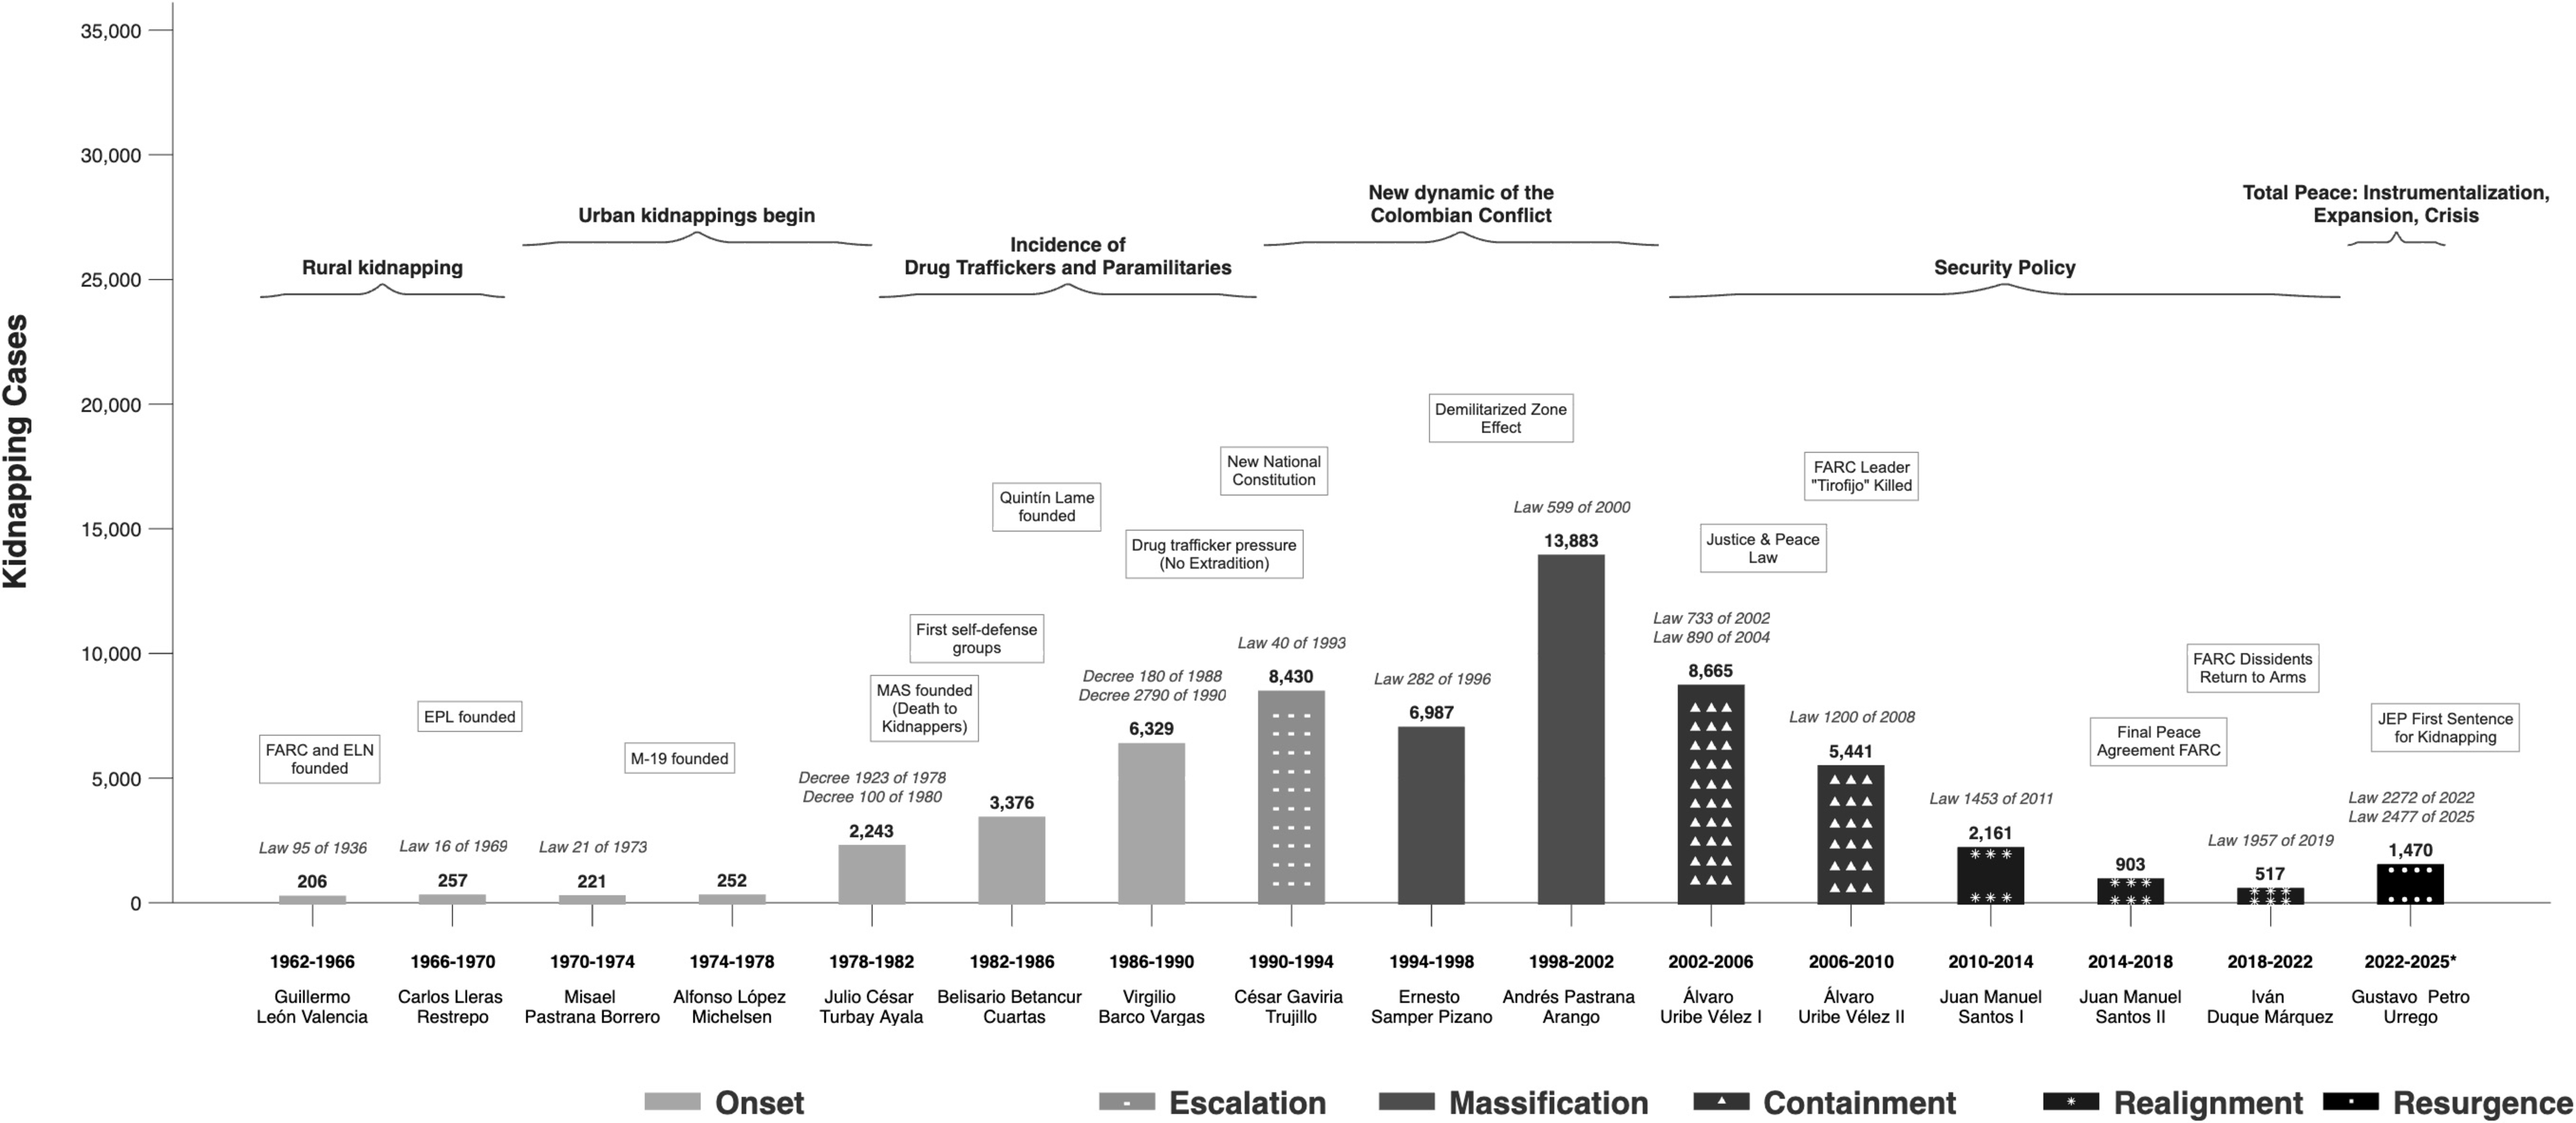
\includegraphics[width=\linewidth]{Fig_4.pdf}
\caption{Evolution of kidnappings in Colombia: armed conflict, security policy, and institutional change (1962--2025).}
\label{fig:evolucion-historica}
\figurenote{\textit{Note:} The figure presents the total number of kidnappings per presidential term in Colombia from 1962 to 2025. Each bar corresponds to a presidential administration; the final period corresponds to partial data from the Gustavo Petro administration. Shading distinguishes phases of the armed conflict, and annotations highlight developments related to armed groups, legal reforms, and security policies. The total reported in this period amounts to 61,341 cases. \textit{Source:} Author's elaboration based on \citet{cnmh_datos} and \citet{pinto2004}.}
\end{figure}

This trajectory culminated in a phase of massification during the administrations of César Gaviria, Ernesto Samper, and especially Andrés Pastrana, when kidnapping reached its highest levels, exceeding 13,000 cases in the 1998--2002 period, as illustrated in Figure~\ref{fig:evolucion-historica}. This critical moment coincided with the promulgation of the 1991 Constitution, pressures from drug cartels, the consolidation of paramilitary structures, and the Caguán demilitarized zone, as well as key legislative measures such as \citet{ley40_1993} and \citet{ley282_1996}, which created a comprehensive regulatory framework and gave birth to the GAULA. From 2002 onward, under the administrations of Álvaro Uribe Vélez, a containment phase is identified, associated with a more assertive security policy and the strengthening of military and police capabilities; laws such as \citet{ley733_2002}, \citet{ley890_2004}, and \citet{ley1200_2008} constituted a framework of criminal toughening aimed at substantially increasing the costs of kidnapping. During the administrations of Juan Manuel Santos, a realignment phase was observed with low levels of kidnapping in the context of the peace process and the signing of the Final Agreement with the FARC; \citet{ley1957_2019} introduced conditional sentence reductions for kidnapping crimes in cases of submission to the Special Jurisdiction for Peace (JEP). In the most recent period, under the government of Gustavo Petro, a moderate resurgence is observed, associated with the fragmentation of armed actors, the re-emergence of dissident groups, and the evolution of conflict dynamics, in a regulatory environment shaped by \citet{ley2272_2022}, which provides for the suspension of arrest warrants for leaders and members of illegal armed groups, including those responsible for serious crimes such as kidnapping. Taken together, the figure suggests that the evolution of kidnapping in Colombia has systematically responded to changes in the political, institutional, and legal environment, indicating that this crime does not follow an autonomous path but is closely tied to the cycles of the armed conflict and the state's capacity to adapt its regulatory and operational framework.

\subsection{Macroeconomic analysis: stochastic trend}

This section provides empirical evidence for the mechanism, not merely a descriptive complement. It establishes that kidnapping for ransom, non-extortionate kidnapping ($K^{NE}$), and the commercial lending rate ($r$) share a common stochastic trend that guarantees the existence of a persistent state environment over which the planner can screen the behavior of types from a macroeconomic perspective. The rate $r$ functions as an indicator of macroeconomic dynamics that sets the opportunity cost and continuation value of the crime, while $K^{NE}$ marks the phase in which the criminal organization accumulates logistical muscle, operational experience, and territorial control, thereby reducing its marginal cost of operation and enabling the more professional and systematic structuring of kidnapping for ransom.

Separating the permanent component of kidnapping for ransom ($K^E$) from its transitory fluctuations requires tools capable of identifying long-run stochastic trends. For this purpose, two conceptually independent econometric frameworks are employed: the Vector Error Correction (VEC) model and the Local Linear Trend (LLT) model. The first exploits cointegration relationships among variables in a multivariate system; the second decomposes the series univariately in state-space. Although constructed from different principles, both converge in identifying the same permanent component of the phenomenon. This result does not reflect one model confirming the other; rather, it illustrates the \emph{equivalence} between stochastic trends: different admissible methods applied to the same $I(1)$ series reveal the same permanent trend space up to a stationary component, as established by Corollary~\ref{cor:equiv-trend} formulated below. The data used are continuous monthly series from July 1954 to December 2025 ($T=858$ observations), obtained from the National Center for Historical Memory \citet{CNMH2013, cnmh_datos}, from official statistics of the Colombian State \citet{mindefensa_stats}, and from the historical series of \citet{banrep_series_historicas}. The VEC specification draws on the literature that models crime as a cointegrated system and on its application to kidnapping and disappearance in Australia and Colombia, as shown by \citet{Masih1995} and \citet{Suarez_2025}.

% ── VEC ──────────────────────────────────────────────────────────────────────

The first framework, the VEC model, characterizes the long-run relationship and the adjustment dynamics among these three series. Augmented Dickey--Fuller (ADF) and KPSS tests place all three series in $I(1)$, and Johansen's cointegration test supports a single cointegrating vector. Let
\[
\tilde{\mathbf{Y}}_t = (K^E_t,\, K^{NE}_t,\, r_t)'
\]
be the monthly vector. The optimal specification is a VEC with 36 lags, selected by the AIC criterion. Ljung--Box tests at twenty lags do not reject the absence of residual autocorrelation at any conventional level; ARCH$(5)$ tests reject homoskedasticity at the 1\% level in the equations for $\Delta K^E_t$ and $\Delta r_t$, but not at the 5\% level in $\Delta K^{NE}_t$ (Appendix~1). This pattern does not bias the point estimators of $\beta$ and $\alpha$, although inference on short-run coefficients should be read cautiously under heteroskedasticity. The non-normalized cointegrating vector is
\begin{equation}
0{,}037\,K^{E}_t - 0{,}072\,K^{NE}_t - 0{,}049\,r_t = \tilde{\varepsilon}_t,
\qquad \tilde{\varepsilon}_t \sim I(0).
\label{eq:vec-coint}
\end{equation}
Normalizing on $K^E_t$, the long-run structural equation is
\begin{equation}
K^E_t = 1{,}93\,K^{NE}_t + 1{,}31\,r_t + \varepsilon_t,
\qquad \varepsilon_t \sim I(0).
\label{eq:vec-longrun}
\end{equation}
The coefficient 1{,}93 indicates that $K^{NE}$ operates as a signal of the accumulation of coercive and organizational capacity: in the long run, a unit increase in this modality is associated with an increase of approximately 1{,}93 units in $K^E$, as the expansion of logistical infrastructure, territorial control, and intimidation reduces the marginal costs of moving toward higher-rent activities. The coefficient 1{,}31 on $r$ captures macroeconomic temperature: increases in $r$ slow the economy and restrict liquidity, raising the financing cost of criminal organizations and incentivizing $K^E$ as an immediate source of income; decreases in $r$, in turn, ease that pressure by accelerating activity and cheapening credit.

The error correction system is
\begin{align}
\Delta K^E_t &= -2{,}94\,\tilde{\varepsilon}_{t-1} +
\sum_{j=1}^{35}\Gamma_{1,j}\Delta \tilde{\mathbf{Y}}_{t-j} + \varepsilon_{1,t}, \label{eq:vec1}\\
\Delta K^{NE}_t &= 0{,}36\,\tilde{\varepsilon}_{t-1} +
\sum_{j=1}^{35}\Gamma_{2,j}\Delta \tilde{\mathbf{Y}}_{t-j} + \varepsilon_{2,t}, \label{eq:vec2}\\
\Delta r_t &= -0{,}06\,\tilde{\varepsilon}_{t-1} +
\sum_{j=1}^{35}\Gamma_{3,j}\Delta \tilde{\mathbf{Y}}_{t-j} + \varepsilon_{3,t}. \label{eq:vec3}
\end{align}
Only the loading on the $\Delta K^E_t$ equation is statistically significant at the 1\% level ($p<0{,}01$); that on $\Delta K^{NE}_t$ is not significant at the 10\% level ($p=0{,}17$), and that on $\Delta r_t$ is marginally significant at the 10\% level ($p=0{,}098$). Given that $\beta_{K^E} = 0{,}037$, the effective adjustment speed is $|\alpha_{K^E} \cdot \beta_{K^E}| \approx 0{,}11$: approximately 11\% of any disequilibrium is corrected each period through adjustments in kidnapping for ransom, which emerges as the main margin of absorption of perturbations in the system.

The decomposition of \citet{GonzaloGranger1995} identifies $k - r = 2$ common stochastic trends:
\begin{align}
f_{1,t} &= 0{,}12\,K^E_t + 1{,}00\,K^{NE}_t, \label{eq:gg1}\\
f_{2,t} &= -0{,}02\,K^E_t + 1{,}00\,r_t, \label{eq:gg2}
\end{align}
and the long-run representation of the system is
\begin{equation}
\begin{pmatrix} K^E_t \\ K^{NE}_t \\ r_t \end{pmatrix}
=
\begin{pmatrix} 1{,}60 & 1{,}09 \\ 0{,}81 & -0{,}13 \\ 0{,}04 & 1{,}02 \end{pmatrix}
\begin{pmatrix} f_{1,t} \\ f_{2,t} \end{pmatrix}
+
\begin{pmatrix} u_{1,t} \\ u_{2,t} \\ u_{3,t} \end{pmatrix},
\qquad \mathbf{u}_t \sim I(0).
\label{eq:gg}
\end{equation}
The factor $f_{1,t}$ captures persistent coercive capacity, dominated by $K^{NE}$, while $f_{2,t}$ reflects permanent macro-financial conditions, as illustrated in Figure~\ref{fig:common-trends}. The loading coefficients of $K^E_t$ (1{,}60 on $f_1$ and 1{,}09 on $f_2$) exceed unity, indicating that $K^E$ amplifies both permanent forces.

\begin{figure}[H]
\centering
\begin{subfigure}[t]{0.48\linewidth}
  \centering
  \panelgraphic{\subfigheight}{Fig_5a.pdf}
  \caption{Gonzalo--Granger common factors}
\end{subfigure}\hfill
\begin{subfigure}[t]{0.48\linewidth}
  \centering
  \panelgraphic{\subfigheight}{Fig_5b.pdf}
  \caption{Kidnapping for ransom and VEC--GG trend}
\end{subfigure}
\caption{Common stochastic trends and kidnapping for ransom.}
\label{fig:common-trends}
\figurenote{\textit{Note:} Panel (a) shows the Gonzalo--Granger common factors ($f_{1,t}$, $f_{2,t}$), July 1954--December 2025. Panel (b) reports the observed series of kidnapping for ransom and the VEC--GG long-run trend, July 1954--December 2025 (estimation sample, $T=858$). \textit{Source:} Author's calculations based on \citet{cnmh_datos} and the National Police of Colombia.}
\end{figure}

% ── LLT ──────────────────────────────────────────────────────────────────────

As an independent contrast, a Local Linear Trend (LLT) model is estimated, which decomposes kidnapping for ransom into a stochastic level trend, a persistent slope, and a cyclical component:
\begin{equation}
\begin{aligned}
\text{Measurement:} \quad & y_t = \tau_t + c_t + \xi_t,
&& \xi_t \sim \mathcal{N}(0,\sigma_\xi^2),
&& \hat{\sigma}_\xi \approx 11{,}96\;(p<0{,}001) \\[6pt]
\text{Trend:} \quad & \tau_t = \tau_{t-1} + b_{t-1} + \eta_t,
&& \eta_t \sim \mathcal{N}(0,\sigma_\eta^2),
&& \hat{\sigma}_\eta \approx 7{,}13\;(p<0{,}001) \\[6pt]
\text{Slope:} \quad & b_t = \textstyle\sum_{j=1}^{8}\phi_j b_{t-j} + \nu_t,
&& \nu_t \sim \mathcal{N}(0,\sigma_\nu^2),
&& \hat{\sigma}_\nu \approx 3{,}51\;(p<0{,}001) \\[6pt]
\text{Cycle:} \quad & c_t = \textstyle\sum_{k=1}^{5}\rho_k c_{t-k} + \kappa_t,
&& \kappa_t \sim \mathcal{N}(0,\sigma_\kappa^2),
&& \hat{\sigma}_\kappa \approx 6{,}77\;(p<0{,}001)
\end{aligned}
\label{eq:llt}
\end{equation}
The significance of $\hat{\sigma}_\eta$ confirms that permanent shocks dominate the long-run level of kidnapping for ransom. The autoregressive structure of order 8 in the slope evidences gradual changes in the growth rate, consistent with slow adjustments in criminal capacity rather than abrupt breaks. The stationary cycle of order 5 captures medium-term fluctuations without distorting the permanent trend. Taken together, the LLT results show that kidnapping for ransom is characterized by a dominant stochastic trend with persistent slope dynamics, complemented by mean-reverting cyclical movements.

The long-run trend estimated by the LLT reproduces the broad movements of kidnapping for ransom: the steady increase prior to the late 1990s, the peak associated with the intensification of the armed conflict, and the subsequent stabilization phase. The quantitative comparison with the VEC--GG trend is shown in Figure~\ref{fig:llt-vec}.

\begin{figure}[H]
\centering
\begin{subfigure}[t]{0.48\linewidth}
  \centering
  \panelgraphic{\subfigheight}{Fig_6a.pdf}
  \caption{Trends estimated by LLT and VEC--GG}
\end{subfigure}\hfill
\begin{subfigure}[t]{0.48\linewidth}
  \centering
  \panelgraphic{\subfigheight}{Fig_6b.pdf}
  \caption{Difference between VEC--GG and LLT trends}
\end{subfigure}
\caption{Equivalence of long-run trends for kidnapping for ransom.}
\label{fig:llt-vec}
\figurenote{\textit{Note:} Panel (a) compares the trends estimated by LLT and VEC--GG, July 1954--December 2025 ($T=858$). Panel (b) shows the difference $d_t$ over the same period. \textit{Source:} Author's calculations based on \citet{cnmh_datos} and the National Police of Colombia.}
\end{figure}

The sustained coherence between both trends is not accidental. The difference between the VEC--GG trend and the LLT trend generates an $I(0)$ stationary residual: the ADF test rejects a unit root at the 1\% level ($p<0{,}01$) and the KPSS test with twelve lags does not reject stationarity at the 5\% level ($p=0{,}07$). Thus, the two estimates do not systematically diverge in the long run and provide the empirical counterpart of the following corollary, proved in Appendix~3:


\begin{corollary}[Equivalence of stochastic trends]\label{cor:equiv-trend}
Let $\{y_t\}$ be a time series integrated of order one, $I(1)$. Suppose the existence of two valid decompositions defined as:
\begin{equation*}
    y_t = P_t^{(1)} + u_t^{(1)} = P_t^{(2)} + u_t^{(2)},
\end{equation*}
where $P_t^{(1)}$ and $P_t^{(2)}$ are integrated processes of order one, and $u_t^{(1)}, u_t^{(2)}$ are stationary $I(0)$ processes. It is concluded that:
\begin{equation*}
    P_t^{(1)} - P_t^{(2)} \sim I(0).
\end{equation*}
Consequently, all valid stochastic trends derived from the same observed series are equivalent up to a stationary component.
\end{corollary}

The corollary establishes that the long-run trend of kidnapping for ransom is unique up to stationary disturbances: the VEC model through the Gonzalo--Granger decomposition and the LLT model in its non-parametric estimation independently reveal the same permanent component of the phenomenon \citet{GonzaloGranger1995}. Convergence does not imply that one model confirms the other; rather, both identify the same underlying stochastic structure, which lends robustness to the characterization of the long run regardless of the methodological framework employed.

The relevance of this analysis for the mechanism model is direct. The long-run equilibrium~\eqref{eq:vec-longrun} establishes that the interest rate is a structural determinant of kidnapping for ransom: periods of monetary contraction and credit restriction raise the cost of capital for criminal organizations, reconfiguring their incentives and pushing toward rent-extraction strategies with more immediate returns. This macroeconomic environment is not neutral with respect to captor types: it defines the support of the cost distribution and the valuation of ransom faced by heterogeneous agents in each period, feeding the parameter space within which the screening mechanism operates. The persistence of the two common trends identified, coercive capacity and macro-financial conditions, implies that heterogeneity across types is not transitory or purely idiosyncratic, but structurally conditioned by the long-run macroeconomic environment. This property justifies its explicit treatment as restrictions on the type support in the mechanism design model developed in Section~\ref{sec:model}.

\subsection{Microstructure and competing hazards in Colombia}\label{sec:empirico}

The macroeconometric analysis in the previous section establishes the long-run trends of kidnapping and its relationship with the lending interest rate, but it does not reveal the micro-level dynamics underlying each individual episode: which type of organization detains the victim, what motivates it to yield or resist, how long the victim remains in captivity, and under what conditions the event is resolved. These elements are indispensable for the mechanism design model, as they define the support of the criminal type distribution, the retention technologies of each group, and the policy elasticities the state can exploit. This section leverages individual microdata from \citet{cnmh_datos} to estimate two complementary models, namely a Multinomial Logit (MNL) and a proportional hazards model of \citet{Cox1972}, whose joint results directly feed the heterogeneous type structure of the screening mechanism.

These microdata come from the Information System on Events of Violence in the Colombian Armed Conflict (SIEVCAC) of the National Center for Historical Memory, which integrates and cross-validates institutional and social sources for each individually documented case. From an initial universe of $N=39,369$ observations, three sequential filters were applied: confirmation of extortionate typology ($n=11,270$, 28.6\%), existence of an observable outcome ($n=1,133$, 10.1\% of the extortionate stratum), and availability of complete covariates, yielding a final analytical sample of $n=1,125$ cases (2.9\% of the total universe). The magnitude of this reduction motivated a sample selection test to determine whether the loss of information on the outcome variable is due to observable factors or is statistically random: a binary logistic model was estimated on the extortionate stratum with complete attrition covariates ($n=11,253$ of $11,270$ extortionate cases with valid date), with the dependent variable equal to one when the outcome is unobservable \citet{LittleRubin2020}. The results reveal that the loss of information follows a systematic pattern. The probability of an unobservable outcome is significantly higher in all non-urban areas (OR between 1.9 and 2.2, $p<0.001$) and during the period of greatest conflict intensity, between 1998 and 2002 (OR$\,=\,$1{,}76, $p=0.001$), thereby ruling out complete randomness in the missingness mechanism. However, the victim's profile and the scale of the kidnapping do not predict the absence of information ($p>0.10$), confirming that the substantive covariates of the model are orthogonal to the selection process. The bias is therefore of territorial representativeness (the sample overrepresents metropolitan events), not of estimation of the structural effects of interest. In summary, the sample selection test indicates that the final analytical sample is \textit{representative of the structural relationships} (armed actor, victim profile, and case structure), but not of the territorial universe of Colombian extortionate kidnapping. As an advantage, the orthogonality between the missingness mechanism and the substantive covariates preserves the internal validity of the estimators. As a limitation, the overrepresentation of metropolitan events restricts the extrapolation of frequencies to peripheral regions and the period of greatest conflict intensity.

On the final analytical sample ($n=1,125$), two model specification verifications were performed, and a substantive contrast result is reported. \textit{(i) Validity of the IIA assumption}: the test evaluates whether the alternatives of the model are mutually independent, a necessary condition for the Multinomial Logit to be the correct estimator; the SUEST generalization of \citet{HausmanMcFadden1984} and \citet{Weesie1999} does not reject this assumption ($\chi^2(1)=0{,}24$, $p=0{,}625$), confirming that the discrete choice structure is correctly specified. \textit{(ii) Stability of the coefficients}: this verification assesses whether the results are sensitive to the researcher's methodological decisions, comparing three specifications of the same model \citet{Wooldridge2010}. The first is the main model with standard errors clustered at the municipal level; the second replaces the cluster with robust standard errors to rule out that the standard errors are artificially inflated by the grouping structure; the third excludes the duration of captivity variable to mitigate its potential endogeneity, given that duration may be jointly determined with the outcome. The robustness criterion is strict: if the coefficients of interest maintain their sign and statistical significance in all three versions, the estimated effects reflect genuine structural relationships rather than artifacts of a particular specification. The result confirms this stability: the effect of common delinquency on the probability of death ($\hat{\beta}\approx 4.15$, $p<0.01$) and that of the collective structure of the kidnapping ($\hat{\beta}\approx 2.46$, $p<0.001$) are invariant across the three specifications, validating the structural interpretation of the estimators. \textit{(iii) Heterogeneity in the cost of criminal failure}: the model reveals that the death rate in captivity differs substantially across organizations: 8{,}0\% in common delinquency compared to 0.2\% in the FARC. The difference-in-proportions test, whose purpose is to determine whether this gap is statistically distinguishable from chance, confirms that the difference is significant ($z=-5{,}71$, $p<0.001$), demonstrating structural heterogeneity among organizations in the cost assumed upon negotiation failure.

Taken together, the three procedures allow a judgment on the analytical quality of the final sample. The model is correctly specified, the estimators are stable under variations in the estimation strategy, and the heterogeneity among organizations is statistically identifiable with the available data, guaranteeing internal validity. The sample of $n=1,125$ cases provides sufficient variation to identify the structural mechanisms of interest, but its territorial scope is limited by the overrepresentation of metropolitan events, which restricts the extrapolation of frequencies to peripheral regions. The balance is therefore favorable for structural inference and restrictive for distributive inference: the estimated effects are reliable, but absolute proportions must be interpreted as lower bounds of the phenomenon in areas of low institutional visibility.

With the sample validated, the two estimated models address complementary dimensions of the same phenomenon. The MNL answers the question \textit{what happens?}: it estimates the relative probability of each outcome (payment, death, rescue, or escape/release without payment) as a function of the perpetrator's profile, the victim, the geographic context, and operational tactics, without incorporating the temporal dimension. The Cox model answers the question \textit{when does it happen?}: it models the instantaneous hazard of resolution of the event as a function of time elapsed in captivity, capturing the speed with which each type of organization closes the process. The complementarity between the two is structural for the analysis: the MNL identifies the distribution of criminal types through differences in conditional outcomes on observable covariates, while the Cox model reveals heterogeneity in retention technologies through differences in the speed of resolution. Together, they allow separating the static dimension of choice from the dynamic dimension of implementation, providing the empirical inputs required by the screening mechanism.

% ── MNL AND COX DIFFERENCES ──────────────────────────────────────────────────

% ── MNL MODEL ────────────────────────────────────────────────────────────────

The Multinomial Logit identifies the determinants of each outcome. With the reference category fixed at Payment ($Y=1$), it estimates the log-odds of each alternative outcome $j\in\{0,2,3\}$ as:
\enlargethispage{3\baselineskip}
{\small\setlength{\abovedisplayskip}{2pt}%
\setlength{\belowdisplayskip}{2pt}%
\setlength{\abovedisplayshortskip}{2pt}%
\setlength{\belowdisplayshortskip}{2pt}%
\begin{equation}
\ln\!\left(\frac{\Pr(Y_{i,m}=j \mid X_{i,m})}{\Pr(Y_{i,m}=1 \mid X_{i,m})}\right)
= \alpha_j
+ \underbrace{G_i'\beta_{1,j}}_{\text{Perpetrator}}
+ \underbrace{V_i'\beta_{2,j}}_{\text{Victim}}
+ \underbrace{C_{i,m}'\beta_{3,j}}_{\text{Context}}
+ \underbrace{T_i'\beta_{4,j}}_{\text{Tactics}},
\quad j\in\{0,2,3\}.
\label{eq:mnl}
\end{equation}
}
The vector $X_{i,m}\in\mathbb{R}^{26}$ comprises indicators of armed group ($G_i$, reference FARC), victim profile ($V_i$, reference high income), geographic zone and historical period ($C_{i,m}$, reference metropolis and pre-1998), and operational modality and captivity duration ($T_i$). Standard errors are clustered at the municipal level (373 units). The model is jointly significant: Wald $\chi^2(78)=5.250{,}34$, $p<0.001$, Pseudo $R^2=0.18$. The complete estimation is reported in Appendix~2.

The MNL produces three findings that structure the type heterogeneity required by the mechanism; in each case, the magnitude is expressed via the relative risk ratio (RRR), which compares the probability of an alternative outcome against Payment as the reference category. \textit{First}, in the post-2011 period, the RRR of Escape without payment is 11.28 times higher than in the pre-1998 period ($p<0.01$), reflecting the collapse of the retention value given the accumulated deterrent capacity of the GAULA \citet{Mejia2000Secuestro}: as state intervention is consolidated, kidnapping for ransom loses economic viability, and the captor releases the victim without demanding ransom. \textit{Second}, for public sector victims, the RRR of Escape is 3.92 times higher than for high-income victims ($p<0.01$); the state policy of non-negotiation renders this segment a financially unviable asset for the captor, who faces a low probability of collection and a persistent risk of intervention without economic counterpart. \textit{Third}, the RRR of Rescue declines monotonically with the duration of captivity, from 0.18 in short-duration captivities to 0.08 in prolonged ones ($p<0.01$): short captivities reach only 18\% and prolonged ones only 8\% of the relative probability of Rescue observed in express kidnappings, which confirms that the state loses operational effectiveness as the captor consolidates its position, and that the tactical intervention window is concentrated in the initial phases of the event. Figure~\ref{fig:mnl-a} illustrates these three patterns simultaneously.

\begin{figure}[H]
\centering
\begin{subfigure}[t]{0.48\linewidth}
  \centering
  \panelgraphic{\subfigheight}{Fig_7a.pdf}
  \caption{State Rescue by captivity duration}
\end{subfigure}\hfill
\begin{subfigure}[t]{0.48\linewidth}
  \centering
  \panelgraphic{\subfigheight}{Fig_7b.pdf}
  \caption{Escape or release without payment by victim profile}
\end{subfigure}
\caption{MNL predicted probabilities: rescue and escape by key covariates.}
\label{fig:mnl-a}
\figurenote{\textit{Note:} Panel (a) reports the probability of state Rescue by captivity duration category. Panel (b) shows the probability of Escape or release without payment by victim profile. \textit{Source:} Author's calculations based on \citet{cnmh_datos}, Stata~19.}
\end{figure}

The geographic dimension and the identity of the perpetrator group provide two additional sources of structural heterogeneity with direct implications for the mechanism design model. In the territorial dimension, the Rescue probability decreases from 0.465 in metropolitan areas and 0.447 in the Andean region to 0.414 in the Pacific, 0.424 in the East/Jungle, and 0.343 in the Caribbean, a gradient that reflects differences in institutional density, logistical accessibility, and the permanent presence of the GAULA in the territory. In the organizational dimension, the unconditional margins of the MNL show that the probability of Death in captivity follows an ordering determined by the logistical retention capacity of each organization: 0.002 for the FARC, 0.007 for the ELN, 0.026 for the paramilitaries, and 0.071 for common delinquency. This gradient confirms that the risk of execution is inversely proportional to such capacity; actors with lesser infrastructure face a shorter time horizon before the failure of the negotiation translates into violence. Figure~\ref{fig:mnl-b} presents both patterns.

\begin{figure}[H]
\centering
\begin{subfigure}[t]{0.48\linewidth}
  \centering
  \panelgraphic{\subfigheight}{Fig_8a.pdf}
  \caption{State Rescue by geographic zone}
\end{subfigure}\hfill
\begin{subfigure}[t]{0.48\linewidth}
  \centering
  \panelgraphic{\subfigheight}{Fig_8b.pdf}
  \caption{Death in captivity by responsible group}
\end{subfigure}
\caption{MNL predicted probabilities: rescue by region and death by perpetrator group.}
\label{fig:mnl-b}
\figurenote{\textit{Note:} Panel (a) reports the probability of state Rescue by geographic zone. Panel (b) shows the probability of Death in captivity by responsible group. \textit{Source:} Author's calculations based on \citet{cnmh_datos}, Stata~19.}
\end{figure}

% ── COX MODEL ────────────────────────────────────────────────────────────────

The second complementary model applies the proportional hazards model of \citet{Cox1972}, estimated under a competing risks framework. Since the outcome can be Payment, Rescue, Death, or Escape/Release, four independent cause-specific models are estimated: in each, the event of interest defines the failure, and the remaining three outcomes are treated as right-censored observations \citet{Bradburn2003}. For event $j\in\{\text{Payment, Rescue, Death, Escape}\}$, the cause-specific hazard is specified as
\begin{equation}
h_j(t \mid X) = h_{0j}(t)\exp\!\left(X'\tilde{\beta}_j\right),
\qquad
S_j(t \mid X) = \exp\!\left(-H_{0j}(t)\exp\!\left(X'\tilde{\beta}_j\right)\right),
\label{eq:cox}
\end{equation}
where $h_j(t\mid X)$ is the instantaneous cause-specific hazard for outcome $j$ at time $t$; $h_{0j}(t)$ is its non-parametric baseline component; $\exp(X'\tilde{\beta}_j)$ is the proportional risk factor; $H_{0j}(t)$ is the cumulative baseline hazard; and $S_j(t\mid X)$ is the probability of not having observed $j$ up to $t$. The vector $X$ replicates the perpetrator, victim, context, and tactics blocks of the MNL, excludes captivity-duration categories, which are collinear with the time axis when resolution time is the dependent variable, and is estimated on the subsample with positive and observed duration ($N=461$). The hazard ratio (HR) quantifies the relative resolution speed of each group with respect to the FARC, which acts as the reference category: HR$>1$ indicates a higher resolution rate than the FARC, and HR$<1$ a lower rate.

The results reveal three findings. \textit{Heterogeneity in retention technologies}: paramilitaries exhibit HR$=4.28$ for Payment ($p<0.001$), that is, they collect the ransom at a rate four times higher than the FARC; common delinquency registers HR$=1.71$ ($p=0.021$), reflecting short negotiation horizons and high turnover. The ELN does not differ significantly ($p=0.317$), confirming operational symmetry with the FARC. \textit{Operational paralysis in public sector victims}: HR of Payment$=0.20$ ($p<0.001$) and of Rescue$=0.24$ ($p=0.001$); values less than one indicate slower resolution than the reference group, rendering this segment an asset with negative expected value for the captor. \textit{Institutional efficiency scissor}: post-2011, the Payment speed falls by 49\% (HR$=0.51$, $p=0.035$) while that of Rescue is multiplied by 4.86 ($p<0.001$), collapsing the profitability of kidnapping for ransom. Figure~\ref{fig:cox-a} shows the amplifying effect of the GAULA: the Rescue probability shifts from 0.64, 0.28, and 0.14 without intervention to 0.72, 0.35, and 0.19 with intervention for express, short, and long captivities.

\begin{figure}[H]
\centering
\begin{subfigure}[t]{0.48\linewidth}
  \centering
  \panelgraphic{\subfigheight}{Fig_9a.pdf}
  \caption{Rescue by GAULA intervention and duration}
\end{subfigure}\hfill
\begin{subfigure}[t]{0.48\linewidth}
  \centering
  \panelgraphic{\subfigheight}{Fig_9b.pdf}
  \caption{Survival of duration by perpetrator}
\end{subfigure}
\caption{Temporal dynamics of rescue and heterogeneity in captivity duration.}
\label{fig:cox-a}
\figurenote{\textit{Note:} Panel (a) reports the probability of Rescue by GAULA intervention and duration category. Panel (b) presents the survival curves of captivity duration by perpetrator group. \textit{Source:} Author's calculations based on \citet{cnmh_datos}, Stata~19.}
\end{figure}

The cumulative Rescue dynamics confirm that state effectiveness varies with the organizational structure of the perpetrator. Toward day 100, the cumulative Rescue probability reaches 0.33 for paramilitaries, 0.29 for the ELN, and 0.27 for the FARC: the greater territorial exposure and more urban operational positioning of paramilitary groups increase their vulnerability to state intervention in the long run. The dynamic mortality profile (Cox margins in Figure~\ref{fig:cox-b}) reproduces the MNL hierarchy: the probability of Death reaches 0.079 in common delinquency and 0.002 in the FARC (approximately forty times higher), compared with the static MNL margins reported above (0.071 and 0.002, approximately thirty-five times), a difference that reflects that the Cox model additionally captures the temporal speed at which the lethal outcome materializes. Figure~\ref{fig:cox-b} presents these patterns.

\begin{figure}[H]
\centering
\begin{subfigure}[t]{0.48\linewidth}
  \centering
  \panelgraphic{\subfigheight}{Fig_10a.pdf}
  \caption{Cumulative state Rescue probability}
\end{subfigure}\hfill
\begin{subfigure}[t]{0.48\linewidth}
  \centering
  \panelgraphic{\subfigheight}{Fig_10b.pdf}
  \caption{Mortality in captivity by perpetrator group}
\end{subfigure}
\caption{Cumulative rescue probability and mortality in captivity by armed group.}
\label{fig:cox-b}
\figurenote{\textit{Note:} Panel (a) shows the cumulative state Rescue probability by armed group, 1964--2025. Panel (b) reports the probability of Death in captivity by perpetrator group. \textit{Source:} Author's calculations based on \citet{cnmh_datos}, Stata~19.}
\end{figure}

\section{Relevance of the Empirical Framework for the Mechanism Model}\label{sec:pertinencia}

The theoretical model in Section~\ref{sec:model} requires two empirical inputs so as not to depend on ad hoc assumptions: a persistent macroeconomic environment that disciplines retention costs and a type structure with differentiated priors, technologies, and hazards. The VEC system, the Gonzalo--Granger decomposition, and Corollary~\ref{cor:equiv-trend} provide the first input. The cointegration among $K^E$, $K^{NE}$, and $r$ establishes that kidnapping for ransom does not evolve as an isolated series, but as part of a long-run system in which coercive capacity and macro-financial conditions act as permanent forces. The equivalence between the VEC--GG trend and the LLT trend prevents calibration from depending on a single econometric specification, while the adjustment structure of the VEC shows that $K^E$ is the margin that absorbs disequilibria. Therefore, the state vector of the mechanism, the feasible set $\Gamma_t(\mu_t)$, and the constraints $IC^K$ and $IR^{K,F}$ are anchored in persistent regularities, not in a purely theoretical normalization.

On this basis, the MNL and the Cox model connect microeconomic evidence with the initial distribution $\mu_0\in\Delta(\ThetaK)$ and the technology vectors $\beta_{K,j}(\theta_K)$. The MNL provides the static fingerprint of each type by relating perpetrator, victim, context, and tactics to the conditional distribution of outcomes; thus, the initial belief and terminal payments are set with observed weights. The Cox model provides the dynamic dimension: its cause-specific hazards are transferred to the mechanism as rates $\lambda_j(\theta_K,t)$ that govern the daily signal $\zeta_t$, update the posterior $\mu_t$, and determine the speed of learning. The empirical separation of those rates across organizations is the observational basis of Lemma~\ref{lem:hazard-separation} and the criterion of \citet{Kakutani1948}: if the trajectories induced by the types generate sufficiently distinct laws, the posterior can concentrate on the true type. Together, the empirical block converts macro and micro data into priors, costs, hazards, and constraints directly usable by the dynamic mechanism. The explicit translation protocol between estimators and structural parameters is detailed at the beginning of Section~\ref{sec:calibracion}.

\section{The Theoretical Model}\label{sec:model}

This section formalizes the mechanism for the deterrence and dismantling of kidnapping for ransom through an indirect approach. While the Revelation Principle of \citet{Gibbard1973} and \citet{Myerson1979IC,Myerson1981} guarantees equivalence with a direct mechanism, a path used by \citet{MyersonSatterthwaite1983} to delimit the efficiency frontier of bilateral exchange, by \citet{Rochet1987} to characterize implementability conditions in quasi-linear environments with multidimensional types, and by \citet{RochetChone1998} to solve the non-linear multidimensional screening problem, this route is not viable here because the captor never voluntarily reveals its type, in line with the incentives to misreport private information of \citet{Fearon1995Rationalist}, and the observable instruments, financial interdiction $\alpha_t\in[0,1]$ and operational pressure $\gamma_t\in[0,1]$, would lose their empirical anchoring by collapsing into abstract messages of revelation. The \emph{Mano de Dios-Guadalupe} (MDG) process operationalizes the indirect approach through a logit noise with a hybrid temperature between the latent strategic intention and the materialized action; in the base specification with a positive residual floor, it guarantees full support across all branches of the game endogenously to the operational dynamics, unlike \citet{Selten1975Perfectness}, \citet{KrepsWilson1982}, and \citet{FudenbergTirole1991}, who achieve the same purpose through external axiomatic perturbations on strategies, belief systems consistent with sequential rationality, and Bayesian update rules in the Perfect Bayesian Equilibrium (PBE). This guarantee of full support is the condition that allows the PBE to discipline beliefs about $\theta_K$ through Bayes' update and sequential consistency, so that the accumulation of public signals generated by asymptotically separable competing risks forces the convergence of the posterior distribution toward the structural identity of the true type, a result formalized in Theorem~\ref{thm:posterior-consistency}.

\subsection{Definition of the mechanism}\label{subsec:def-mecanismo}

Let $\mathcal{J}=\{S,K,F\}$ be the set of players, where $S$ represents the state, $K$ the captor, and $F$ the family. Each episode is characterized by the vector of types $\theta=(\theta_K,\theta_F,\theta_V,\theta_S)\in\Theta$, where $\ThetaK=\{\text{DC},\text{PAR},\text{ELN},\text{FARC}\}$ corresponds to the captor's type, namely, common delinquency, paramilitary groups, National Liberation Army, and Revolutionary Armed Forces of Colombia; $\Theta_F=\{\text{High},\text{Low}\}$ represents the family's payment capacity; $\Theta_V=\{\text{Public},\text{Private}\}$ represents the victim's profile; and $\Theta_S=\{\text{Hard},\text{Lax}\}$ represents the institutional environment. Each episode is also localized in an observable geographic zone $z\in\mathcal{R}$, where $\mathcal{R}$ groups five regions (Metropolitan, Andean, Caribbean, Pacific, and East-Jungle); $z$ is not a private strategic type but a public initial condition that disciplines the prior over the captor's type. Only $\theta_K$ is private information of $K$; the other components and $z$ are observable upon opening the episode, with an initial belief $\mu_0(\theta\mid z,\theta_V)=\Prob(\theta_K=\theta\mid z,\theta_V)\in\Delta(\ThetaK)$.


The public history $h_t\in H_t$ recursively records, up to the beginning of $t$ and without including the type vector $\theta$ or the belief $\mu_t$, the following elements: $t$ is the period index; $\alpha^\ast_{[0,t-1]}$ and $\gamma^\ast_{[0,t-1]}$ are the trajectories of the state's financial interdiction and operational pressure instruments; $\tilde{a}^F_{[0,t-1]}$, $\tilde{a}^K_{[0,t-1]}$, and $\tilde{a}^S_{[0,t-1]}$ are the actions executed by the family, the captor, and the state; $m_{[0,t-1]}$ is the sequence of physical outcomes; and $d_{[0,t-1]}$ is the sequence of institutional detection signals, where $d_t\in\{0,1\}$ indicates whether in period $t$ the state detected collusion between the family and the captor, i.e., a clandestine ransom payment bypassing the financial interdiction policy.
\begin{gather}
h_t = \bigl(t,\,\alpha^\ast_{[0,t-1]},\,\gamma^\ast_{[0,t-1]},\,\tilde{a}^F_{[0,t-1]},\,\tilde{a}^K_{[0,t-1]},\,\tilde{a}^S_{[0,t-1]},\,m_{[0,t-1]},\,d_{[0,t-1]}\bigr),\label{eq:historia-publica}\\
h_{t+1} = \bigl(h_t,\,\alpha_t^\ast,\,\gamma_t^\ast,\,\tilde{a}_t^F,\,\tilde{a}_t^K,\,\tilde{a}_t^S,\,m_t,\,d_t\bigr).\label{eq:actualizacion-historia}
\end{gather}
The information sets when choosing in $t$ are
\begin{gather*}
\mathcal{I}_t^S=\bigl(h_t,z,\theta_F,\theta_V,\theta_S,\mu_t\bigr),\\
\mathcal{I}_t^F=\bigl(h_t,z,\theta_F,\theta_V,\theta_S\bigr),\qquad
\mathcal{I}_t^K=\bigl(h_t,z,\theta_K,\theta_F,\theta_V,\theta_S\bigr).
\end{gather*}
Although $\mu_t$ is internal to the state, its exclusion from the private information sets does not generate inconsistency: in the PBE, private agents share the same prior and the same public history $h_t$, and therefore replicate the Bayesian updating of the planner \citet{FudenbergTirole1991}.

The space of institutional allocations of the state is $\mathcal{X}_t=\mathcal{A}^{S,\mathrm{disc}}\times\mathcal{A}^{\alpha}\times\mathcal{A}^{\gamma}$. In each period $t$, players formulate optimal strategic intentions $a_t^{i\ast}$; the MDG process transforms them into executed actions $\tilde{A}_t=(\tilde{a}_t^F,\tilde{a}_t^K,\tilde{a}_t^S)$ that enter the public registry and determine $h_{t+1}$ and the public signal $\zeta_t$. Conditional on the executed actions and the optimal institutional policy, the system determines the physical outcome $m_t\in\mathcal{M}_{\mathrm{out}}$ through a block of competing risks, with $\mathcal{M}_{\mathrm{cont}}=\{\mathrm{cont}\}$, $\mathcal{M}_{\mathrm{term}}=\{\mathrm{pay},\mathrm{res},\mathrm{rel},\mathrm{kill}\}$, and $\mathcal{M}_{\mathrm{out}}=\mathcal{M}_{\mathrm{cont}}\cup\mathcal{M}_{\mathrm{term}}$.

The horizon of the episode is not fixed in advance but is determined by the captivity dynamics themselves: the episode concludes in the first period in which a terminal outcome materializes, so the effective horizon is the endogenous stopping time
\begin{equation}
\tau=\inf\{t\geq 0:m_t\in\mathcal{M}_{\mathrm{term}}\},\label{eq:stopping-time}
\end{equation}
where the recursive construction of $h_t$ ensures that the event $\{\tau=t\}$ is measurable with respect to the public history at the beginning of $t$, guaranteeing that the state recognizes the closure of the episode in real time. On these elements, with $\mathbb{T}=\{0,1,\ldots,\tau\}$ as the active periods index, $\Theta=\ThetaK\times\Theta_F\times\Theta_V\times\Theta_S$ the type space, $(H_t)_{t\in\mathbb{T}}$ the family of public history spaces recursively generated by~\eqref{eq:historia-publica}--\eqref{eq:actualizacion-historia}, $(\mu_t)_{t\in\mathbb{T}}$ the belief process in $\Delta(\ThetaK)$ updated by Bayes' rule throughout the episode, and $\Prob$ the ex-ante law induced by the strategy profile $s$, the prior $\mu_0$, and the captivity dynamics, the dynamic mechanism of kidnapping deterrence is formally defined as the tuple
\[
\mathcal{D}=\bigl\langle\mathcal{J},\,\mathbb{T},\,\Theta,\,\mathcal{R},\,(\mathcal{X}_t)_{t\in\mathbb{T}},\,(H_t)_{t\in\mathbb{T}},\,(\mu_t)_{t\in\mathbb{T}},\,\Prob\bigr\rangle.
\]
Given $z\in\mathcal{R}$ and $\theta_K\sim\mu_0$, the state's strategy $s^S=\chi=(\chi_t)_{t\in\mathbb{T}}$ is implemented via the measurable public policy rule $\chi_t\colon H_t\times\mathcal{R}\to\mathcal{A}^{S,\mathrm{disc}}\times\mathcal{A}^{\alpha}\times\mathcal{A}^{\gamma}$, which interacts with the private responses of $K$ and $F$ in their information sets; the social choice rule is formalized by the measurable mapping $f_t\colon\mathcal{I}_t^S\to\mathcal{X}_t$, such that the policy vector in equilibrium is $x_t^\ast:=f_t(\mathcal{I}_t^S)=(a_t^{S\ast},\alpha_t^\ast,\gamma_t^\ast)\in\mathcal{X}_t$. This rule is implementable if it constitutes the path of a PBE in the sense of \citet{FudenbergTirole1991}, which guarantees that the captor cannot systematically induce the state to calibrate its pressure on a type that is not the true one; implementability is achieved when the pair $(s,\mu)$, with $s=(s^S,s^K,s^F)$ and $\mu_t\in\Delta(\ThetaK)$, satisfies two conditions in every reachable information set: \emph{sequential rationality}, whereby each agent $i\in\{K,F\}$ maximises $\mathcal{U}_t^i$ given $\mathcal{I}_t^i$ and the strategies of the others while the state minimizes the expected social loss weighted by $\mu_t$; and \emph{Bayesian consistency}, whereby in every node reached with positive probability under $\Prob^s$, the beliefs satisfy
\[
\mu_t(\theta)=\Prob^s\!\bigl(\theta_K=\theta\mid\mathcal{F}_t^{\mathrm{pub}}\bigr),\qquad \mathcal{F}_t^{\mathrm{pub}}=\sigma\bigl(z,\zeta_0,\ldots,\zeta_{t-1}\bigr),
\]
where $\mathcal{F}_t^{\mathrm{pub}}$ is the public filtration at the beginning of $t$, generated by the $\sigma$-algebra of the initial geographic location $z$ and the public signals $\zeta_0,\ldots,\zeta_{t-1}$; each signal $\zeta_s=(\alpha_s^\ast,\gamma_s^\ast,\tilde{a}_s^F,\tilde{a}_s^K,\tilde{a}_s^S,m_s,d_s)$ aggregates all observables of period $s$ and constitutes the informational support over which the state updates its beliefs about $\theta_K$; so that the instruments $(\alpha_t^\ast,\gamma_t^\ast)$ are calibrated on correct inferences about the captor's type.

\subsection{Summary of the mechanism}\label{subsec:resumen-mecanismo}

In each active period $t$, the protocol advances in three sequential stages. In the first, the agents formulate their optimal intentions: the state resolves $x_t^\ast=f_t(\mathcal{I}_t^S)$, and private agents select their best responses in their respective information sets, conditioned on the observable public policy $(\alpha_t^\ast,\gamma_t^\ast)$ signaled by the state. In the second, the MDG process transforms these intentions into executed actions $\tilde{A}_t$, guaranteeing full support across all branches of the game. In the third, the material state of the episode
\[
\mathcal{C}_t(\theta_K)=\bigl(\theta_K,\theta_F,\theta_V,\theta_S,z,\tilde{a}_t^F,\tilde{a}_t^K,\tilde{a}_t^S,\alpha_t^\ast,\gamma_t^\ast,p_{\mathrm{det},t}\bigr),
\]
with $p_{\mathrm{det},t}$ as the logit probability of detecting collusion, which is increasing in the state's instruments. This material state feeds a block of competing risks that determines $m_t$ and $d_t$; the public signal $\zeta_t$ aggregates all observables of the period and updates the history to $h_{t+1}$ and the belief to $\mu_{t+1}$ through Bayes' rule.

\subsection{Probabilistic technology}\label{subsec:prob-tech}

This section formalizes the stochastic architecture that transforms strategic plans into observable realizations. In the base specification, the MDG process takes as input the latent strategic intention $a_t^{i\ast}$ and generates an executed action $\tilde{a}_t^i$ through an implementation law concentrated on the plan, but with full support over $\mathcal{A}^i$. The executed profile $\tilde{A}_t=(\tilde{a}_t^K,\tilde{a}_t^S,\tilde{a}_t^F)$ is the observable variable that enters the public record, while the strategic intention remains latent. Given $a_t^{i\ast}\in\mathcal{A}^i$ and the state vector $X_t$, execution is determined by
\[
\tilde{a}_t^i\sim\ProbI{i}\bigl(\cdot\mid a_t^{i\ast},X_t\bigr),
\]
and, for each agent $i\in\{K,S,F\}$ and action $a\in\mathcal{A}^i$, it is specified as
\begin{equation}
\ProbI{i}\bigl(\tilde{a}_t^i=a\mid a_t^{i\ast},X_t\bigr)
=\frac{\exp\bigl(\mathbf{1}\{a=a_t^{i\ast}\}/T_t\bigr)}{\sum_{a'\in\mathcal{A}^i}\exp\bigl(\mathbf{1}\{a'=a_t^{i\ast}\}/T_t\bigr)},
\label{eq:mdg}
\end{equation}
where $T_t>0$ in the base specification is the temperature of the system: it measures the implementation friction of the episode, not the agent's uncertainty about its own type. To capture strategic learning and institutional maturation jointly, define
\begin{equation}
T_t=T_0\max\Bigl\{\frac{H(\mu_t)}{H(\mu_0)}e^{-\eta_{\mathrm{cal}}t},\,\underline{c}\Bigr\},
\label{eq:temperature}
\end{equation}
with $T_0>0$ as the initial temperature, $\eta_{\mathrm{cal}}>0$ the calendar decay rate, $H(\mu_t)=-\sum_\theta\mu_t(\theta)\ln\mu_t(\theta)$ the entropy of \citet{Shannon1948}, and $\underline{c}\in[0,1]$ the floor of structural noise. In the base specification, the logit distribution~\eqref{eq:mdg} satisfies dominance, full support, and maximum entropy of \citet{Shannon1948} subject to those constraints; under the characterization theorem of \citet{Jaynes1957Information}, this functional form is the entropic maximizer. Dominance concentrates most of the mass on $a_t^{i\ast}$, while every alternative action retains strictly positive probability as implementation friction. Thus, the MDG fulfills a function equivalent, on the operational plane, to the trembling hand of \citet{Selten1975Perfectness} and the sequential evaluation system of \citet{KrepsWilson1982}: no branch of the game is excluded by construction, and beliefs can be updated by Bayes at reached information sets, in line with the consistency of \citet{FudenbergTirole1991PBE}.

Bounded institutional maturation makes the informational component of the noise decline as the system accumulates information, although the structural floor $\underline{c}$ persists. When $\underline{c}>0$, even if $H(\mu_t)\to 0$ the probability of executing exactly $a_t^{i\ast}$ remains strictly less than one: the floor preserves full support over $\mathcal{A}^i$ and no branch is excluded in the limit. The special case $\underline{c}=0$ is interpreted as a limit without residual noise: it allows full convergence $\Prob(\tilde{a}_t^i=a_t^{i\ast}\mid\mathcal{F}_t^{\mathrm{pub}})\to 1$ when $H(\mu_t)\to 0$, but sacrifices that full support. The base version with $\underline{c}>0$ aligns with the absolute continuity or ``grain of truth'' condition of \citet{KalaiLehrer1993}, according to which rational learning must not assign zero probability to events that can occur.

The physical outcome $m_t$ is an observable categorical variable on the support $\mathcal{M}_{\mathrm{out}}$, where $\mathrm{cont}$ represents the continuation of captivity and the four causes of closure are: $j=1$ payment of the ransom by the family, $j=2$ death of the victim in captivity, $j=3$ tactical rescue by the state, and $j=4$ an exogenous residual closure channel with constant baseline intensity $\lambda_4>0$, which groups voluntary release by the captor without formal ransom, logistical fatigue, and administrative truncations of the sample. Conditional on the captor's type and the material state $\mathcal{C}_t(\theta_K)$, its distribution is obtained from the effective intensities $\tilde{\lambda}_j(t\mid\theta_K)$. Denote by
\[
Q_t(m\mid\theta_K,\mathcal{C}_t,\alpha_t^\ast,\gamma_t^\ast)
:=\Prob(m_t=m\mid\theta_K,\mathcal{C}_t,\alpha_t^\ast,\gamma_t^\ast)
\]
the physical outcome transition kernel, and by $\mathsf{G}_t$ the measurable rule that materializes a concrete realization of $m_t$ from that kernel and a uniform draw. The probability that captivity continues at the end of the period is
\[
Q_t(\mathrm{cont}\mid\theta_K,\mathcal{C}_t,\alpha_t^\ast,\gamma_t^\ast)=\exp\!\Bigl(-\sum_{j=1}^{4}\tilde{\lambda}_j(t\mid\theta_K)\,\Delta t\Bigr),
\]
when the episode closes, the cause is drawn with relative weight $\xi_j(t\mid\theta_K)=\tilde{\lambda}_j/\sum_{\ell=1}^{4}\tilde{\lambda}_\ell$, so that causes with higher intensity concentrate the highest probability of materializing. The physical outcome $m_t$ and the detection indicator $d_t$ form $Y_t=(m_t,d_t)\in\mathcal{M}_{\mathrm{out}}\times\{0,1\}$, the projection of $\zeta_t$ onto its last two coordinates. This reduction does not restrict the state's learning, since $\mu_t$ is updated with the complete $\zeta_t$, where $(\alpha_t^\ast,\gamma_t^\ast)$ and $\tilde{A}_t$ enter via the implementation likelihood and the material state $\mathcal{C}_t$. Its function is to isolate the stochastic draw of the competing risks block, whose central objects, intensities $\tilde{\lambda}_j$, \textit{hazards} $\bar{h}_j(t)$, and causal mixture $\xi_j(t)$, are fully determined, conditional on $\mathcal{C}_t$, by the daily law of $Y_t$.

The modeling of risk intensities starts from distinguishing between the instantaneous intensity and its daily probabilistic projection, in line with the proportional hazards tradition of \citet{Cox1972}. The cause-specific intensity $\lambda_j(t)$ measures the marginal propensity to close due to cause $j$ as a rate of occurrence per unit of time; thus, it can take any positive value and is not bounded by one. The discrete hazard $\bar h_j(t)\in[0,1]$, on the other hand, is the probability that event $j$ materializes during interval $t$ conditional on the system having survived to the beginning of the period. The bar in $\bar h_j(t)$ distinguishes this marginal hazard from the public history $h_t$. Both objects depend on the vector of executed actions $\tilde{A}_t$ generated by the MDG process and not on the latent strategic intentions; the state's continuous instruments $(\alpha_t^\ast,\gamma_t^\ast)$ modify them through the material state $\mathcal{C}_t(\theta_K)$.

For each cause $j\in\{1,2,3\}$, the cause-specific intensity adopts a proportional hazards specification conditioned on the material state $\mathcal{C}_t(\theta_K)$:
\begin{equation}
\lambda_j(t\mid\mathcal{C}_t)=\lambda_{j0}(t)\exp(x_t'\beta_j),
\label{eq:lambda-j}
\end{equation}
where $\lambda_{j0}(t)\ge 0$ is the baseline risk of cause $j$, $x_t$ is a design vector encoding the state and action space $(\theta_F,\theta_V,\theta_S,\theta_K,z,\tilde{A}_t,\alpha_t^\ast,\gamma_t^\ast,p_{\mathrm{det},t})$, and $\beta_j$ contains the latent type-specific effect $\beta_{K,j}(\theta_K)$ that captures contrasts in criminal technology across organizations. The termination dynamics decompose into four channels: the three strategic causes $j\in\{1,2,3\}$ linked to institutional design and a fourth intensity $\lambda_4>0$ of exogenous residual closure that groups voluntary release by the captor without formal ransom, logistical fatigue, and administrative truncations of the sample; its intensity is constant baseline and invariant to type $\theta_K$, so its likelihood factorizes orthogonally from the structural parameters in the sense of \citet{Lancaster1990} and \citet{AbbringVanDenBerg2003}. The maturation filter $M(t)=\min\{1,(t/T_{\mathrm{mad}})^2\}\in[0,1]$ scales the strategic intensities to isolate the logistical inertia of the first days of captivity. In discrete time, probabilistic closure cannot be obtained by summing individual transformations $1-\exp(-\lambda_j)$ because that sum may exceed unity; closure is obtained by first aggregating the intensities and then projecting period survival through the aggregated exponential. The effective intensities are:
\begin{equation}
\tilde{\lambda}_j(t\mid\mathcal{C}_t)=M(t)\lambda_j(t\mid\mathcal{C}_t)\;(j=1,2,3),\qquad\tilde{\lambda}_4(t)=\lambda_4,\qquad\Delta t=1.
\label{eq:hj}
\end{equation}
The continuation probability, the daily closure rate, and the conditional distribution of causes are obtained from:
\begin{align}
p_{\mathrm{Cont},t} &= \exp\!\Bigl(-\sum_{j=1}^{4}\tilde{\lambda}_j(t)\Bigr),\label{eq:pCont}\\
q(t) &= 1-p_{\mathrm{Cont},t},\label{eq:q}\\
\xi_j(t) &= \frac{\tilde{\lambda}_j(t)}{\sum_{\ell=1}^{4}\tilde{\lambda}_\ell(t)},\quad j=1,\ldots,4,\label{eq:xi}
\end{align}
so that $\bar h_j(t)=q(t)\xi_j(t)$ is the marginal hazard of cause $j$ and $\sum_j \bar h_j(t)=q(t)\leq 1$ by construction. The probability $\xi_j(t)$ acts as the market share of each risk and orthogonalizes two dimensions of the process: the governance of duration (the when), determined by the aggregate density of the intensities, and the governance of the nature of the closure (the how), governed by the relative weights. It is through $\xi_j(t)$ that Bayesian learning exerts its strategic role: as $\mu_t$ concentrates on the true type, the probability mass is redistributed among exit causes, shifting the likelihood toward the outcomes that are more probable under that type, without altering the temporal scale of captivity. The probability of detecting collusion $p_{\mathrm{det},t}$ is specified through a logistic response function conditioned on the state's instruments:
\begin{equation}
p_{\mathrm{det},t}(\theta_K)=\Lambda(\eta_0(\theta_K)+\eta_1\alpha_t^\ast+\eta_2\gamma_t^\ast),\qquad\Lambda(u)=\frac{1}{1+\exp(-u)}.
\label{eq:detection}
\end{equation}
where $\eta_0(\theta_K)$ is the type-specific intercept that captures the baseline detectability of the criminal organization. Because different organizations differ in their propensity to use traceable formal financial channels, $d_t$ is informative about $\theta_K$. The parameters $\eta_1>0$ and $\eta_2>0$ capture the marginal effect of the financial block and operational pressure. The logistic function guarantees $p_{\mathrm{det},t}(\theta_K)\in(0,1)$ and monotonicity increasing in $(\alpha_t^\ast,\gamma_t^\ast)$: greater financial interdiction or operational pressure raises the probability of observing $d_t=1$, with a baseline level that varies according to the type's concealment technology.

To operationalize the informative quality in rescue planning, the precision index $\iota_t$ is defined as the probability mass of the modal type,
\begin{equation}
\iota_t=\max_{\theta\in\ThetaK}\mu_t(\theta),\qquad\hat{\theta}_t=\operatorname*{arg\,max}_{\theta\in\ThetaK}\mu_t(\theta),
\label{eq:iota}
\end{equation}
where $\hat{\theta}_t$ is the captor's estimated profile. Let $s_t\in\{0,1\}$ be the binary indicator of victim survival at the end of the operational margin of the period, where $s_t=1$ means that the victim survives and $s_t=0$ that she does not survive; this indicator operates in the rescue branch and does not redefine the categorical support of $m_t$. Conditional on a focal rescue attempt, the scalar probability of survival $p_{\mathrm{surv},t}$ is modeled through a logistic response that penalizes the misalignment between the estimated profile and the true type:
\begin{equation}
p_{\mathrm{surv},t}(\iota_t,\hat{\theta}_t,\theta_K):=\Lambda\bigl(\alpha_{\mathrm{leth}}(\theta_K)+\beta_R\cdot\iota_t\cdot\mathbb{1}\{\hat{\theta}_t=\theta_K\}\bigr),
\label{eq:p-surv}
\end{equation}
where $\alpha_{\mathrm{leth}}(\theta_K)$ is the intrinsic lethality of the type, $\beta_R>0$ is the productivity of accumulated intelligence, and $\mathbb{1}\{\hat{\theta}_t=\theta_K\}$ indicates whether the state has correctly identified the captor. When the identification is correct, $\iota_t$ enhances $p_{\mathrm{surv},t}$ according to $\beta_R$; when there is an identification error, the accumulated intelligence becomes inoperative, and the survival probability collapses to the baseline level determined by $\alpha_{\mathrm{leth}}(\theta_K)$.

The daily decision mechanism is projected onto a longitudinal framework via the episode survival function $S(t)$ and the cumulative incidence functions $F_j(t)$. $S(t)$ denotes the probability that the episode remains active until the end of period $t$, and $F_j(t)$ measures the cumulative probability of closure by cause $j$ up to that same horizon. With $S(0)=1$, these objects are constructed as
\begin{equation}
S(t)=\prod_{t'=1}^{t}p_{\mathrm{Cont},t'},\qquad F_j(t)=\sum_{t'=1}^{t}\bar h_j(t')\,S(t'-1),\qquad S(t)+\sum_{j=1}^{4}F_j(t)=1.
\label{eq:longitudinal}
\end{equation}
The constraint $S(t)+\sum_j F_j(t)=1$ guarantees the accounting consistency of the system: all probability not assigned to the continuation of the episode is distributed among the four causes of closure. By weighting each marginal hazard $\bar h_j(t')$ by the remaining survival $S(t'-1)$, the system operates under the formal treatment of competing risks and operationalizes the state's strategic dilemma between intervening immediately or delaying action to accumulate informational capital $\iota_t$.

The technical probability of capture is modeled via a logistic response that keeps the probability within the unit interval and allows public instruments to smoothly modify the marginal effectiveness of the intervention:
\begin{equation}
p_{\mathrm{cap}}(a,\theta_i,\theta_S,\alpha_t^\ast,\gamma_t^\ast)=\Lambda\bigl(\delta_a+c_0(\theta_i)+c_\alpha(\theta_i)\alpha_t^\ast+c_\gamma(\theta_i)\gamma_t^\ast+c_S(\theta_S)\bigr),
\label{eq:p-cap}
\end{equation}
where $\delta_a$ captures the impact of the executed intervention mode itself, $c_0(\theta_i)$ allows for baseline heterogeneity by type, $c_\alpha(\theta_i)$ and $c_\gamma(\theta_i)$ capture how the financial block and operational pressure alter the probability of capture against that specific type, and $c_S(\theta_S)$ incorporates the institutional capacity of the state. The effective probability of capture is defined as the expectation of $p_{\mathrm{cap}}$ over the stochastic realizations of the executed state action, conditional on the tuple $\mathcal{Q}_t^{\mathrm{Cap}}:=(a_t^{S\ast},\alpha_t^\ast,\gamma_t^\ast,\theta_K,\theta_S)$:
\begin{align}
\tilde{p}_{\mathrm{cap},t}(\theta_i)
&:=\E_{\tilde{a}_t^S\mid\mathcal{Q}_t^{\mathrm{Cap}}}\!\bigl[p_{\mathrm{cap}}(\tilde{a}_t^S,\theta_i,\theta_S,\alpha_t^\ast,\gamma_t^\ast)\bigr]\nonumber\\
&=\sum_{a\in\mathcal{A}^S}\ProbI{S}(a\mid a_t^{S\ast},X_t)\cdot p_{\mathrm{cap}}(a,\theta_i,\theta_S,\alpha_t^\ast,\gamma_t^\ast),
\label{eq:p-cap-tilde}
\end{align}
where $\mathcal{Q}_t^{\mathrm{Cap}}$ collects the optimal intention of the state, the executed instruments, and the relevant types of the episode. This formulation separates two levels: $\ProbI{S}$ describes the probability that the state's intention is translated into a concrete action through the MDG process, and $p_{\mathrm{cap}}$ measures the technical probability of capture under the instruments actually executed; in this way, $\tilde{p}_{\mathrm{cap},t}(\theta_i)$ combines implementation uncertainty and operational capacity, avoiding mechanically identifying the planned decision with the observable police outcome.

The mechanism incorporates an additional source of information through micro-level acoustic evidence and learning by absence of communication. In each period $t$, the state can observe a voice window or face operational silence. When there is a signal, it is summarized in a feature vector $x_t^{obs}\in\mathbb{R}^k$ that decomposes the observed signal into the true acoustic pattern of the type ($x_t^{true}(\theta_K)$), channel noise ($\varepsilon_L$), and strategic camouflage ($\varepsilon_S$), with both perturbations being Gaussian and independent of each other:
\begin{equation}
x_t^{obs}=x_t^{true}(\theta_K)+\varepsilon_L+\varepsilon_S,\qquad\varepsilon_L\sim\mathcal{N}(0,\Sigma_L),\quad\varepsilon_S\sim\mathcal{N}(0,\Sigma_S),\quad\varepsilon_L\perp\varepsilon_S.
\label{eq:voz-descomp}
\end{equation}
The Bayesian architecture of the mechanism rests on four likelihoods that convert each observed day into evidence about the captor's type $\theta_K$. The first captures the information contained in executed actions as realizations of the MDG process ($\mathcal{L}_{I,t}$); the second and third collect the information from the physical outcome $m_t$ and the detection signal $d_t$ through the competing risks block; and the fourth incorporates acoustic evidence or operational silence through the communication likelihood $\mathcal{L}_{C,t}$. Analogously to the job search models of \citet{McCall1970}, a continuation day updates the posterior by non-occurrence and a closure updates it through its cause, so that the model converts each observable realization into statistical information without requiring an additional observational layer. The implementation likelihood is the first of these four sources:
\begin{equation}
\mathcal{L}_{I,t}(\theta_K):=\prod_{i\in\{F,K,S\}}\ProbI{i}\!\bigl(\tilde{a}_t^i\mid a_t^{i\ast}(\theta_K),X_t\bigr),
\label{eq:LI-atilde}
\end{equation}
where $a_t^{K\ast}$ may depend directly on $\theta_K$, while $a_t^{F\ast}$ and $a_t^{S\ast}$ depend on the public history and on $\mu_t$; if an executed action was unlikely under the plan induced by a type, that type receives lower posterior weight.

The likelihood of the physical outcome $m_t$ distinguishes two regimes. On a continuation day no competing risk materializes and the absence of closure favors types whose exit rates predict greater continuity:
\begin{equation}
\mathcal{L}_H^{\mathrm{cont}}(t\mid\theta_K)=p_{\mathrm{Cont},t\mid\theta_K}=\exp\!\Bigl(-\sum_{j=1}^{4}\tilde{\lambda}_j(t\mid\theta_K)\Delta t\Bigr).
\label{eq:LH-cont}
\end{equation}
When the day ends due to cause $j^\ast\in\{1,2,3,4\}$, the outcome identifies the type by the cause that produced it:
\begin{equation}
\mathcal{L}_H^{\mathrm{out}}(t,j^\ast\mid\theta_K)=\bar h_{j^\ast}(t\mid\theta_K).
\label{eq:LH-out}
\end{equation}
Let $g:\{1,2,3,4\}\to\mathcal{M}_{\mathrm{term}}$ be the bijection $g(1)=\mathrm{pay}$, $g(2)=\mathrm{kill}$, $g(3)=\mathrm{res}$, $g(4)=\mathrm{rel}$. Both regimes are written as a single expression:
\begin{equation}
\Prob(m_t\mid\theta_K,\mathcal{C}_t)=p_{\mathrm{Cont},t\mid\theta_K}^{\,\mathbf{1}\{m_t=\mathrm{cont}\}}\prod_{j=1}^{4}\bar h_j(t\mid\theta_K)^{\,\mathbf{1}\{m_t=g(j)\}},
\label{eq:LH-compacta}
\end{equation}
a five-cell multinomial ($\mathrm{cont}$ and $\mathcal{M}_{\mathrm{term}}$) where $g$ converts index $j$ into the label of $m_t$.

Regardless of the physical outcome, the detection signal $d_t$ provides a second source of information with Bernoulli likelihood:
\begin{equation}
\Prob(d_t\mid\theta_K,\alpha_t^\ast,\gamma_t^\ast)=p_{\mathrm{det},t}(\theta_K)^{\,d_t}\bigl(1-p_{\mathrm{det},t}(\theta_K)\bigr)^{1-d_t}.
\label{eq:Ld-bernoulli}
\end{equation}

The mechanism incorporates a third source of information through micro-level acoustic evidence and learning by absence of communication. Each type $\theta_K$ possesses a reference profile $(\bar{x}(\theta_K),\Sigma(\theta_K))$; the diagonal Gaussian likelihood assigns greater weight to types whose profiles make the observed signal more plausible:
\begin{equation}
\mathcal{L}_{\mathrm{voz},t}(\theta_K)\propto\exp\!\left(-\frac{1}{2}\sum_{i=1}^{k}\frac{\bigl(x_{t,i}^{obs}-\bar{x}_i(\theta_K)\bigr)^2}{\tilde{\sigma}_i(\theta_K)^2}\right).
\label{eq:Lvoz}
\end{equation}
Let $V_t\in\{0,1\}$ be the indicator of voice emission at $t$ and $\pi_{\mathrm{call}}(\theta_K)\in(0,1)$ the contact probability of each type, interpreted as logistical urgency; both the call and silence are informative. The type-conditional communication likelihood is
\begin{equation}
\mathcal{L}_{C,t}(\theta_K\mid V_t)=\begin{cases}\bigl[\mathcal{L}_{\mathrm{voz},t}(\theta_K)\,\pi_{\mathrm{call}}(\theta_K)\bigr]^{\omega_{\mathrm{voz}}}, & V_t=1,\\[0.5em]\bigl[1-\pi_{\mathrm{call}}(\theta_K)\bigr]^{\omega_{\mathrm{voz}}}, & V_t=0,\end{cases}
\label{eq:LC}
\end{equation}
where $\omega_{\mathrm{voz}}\in[0,1]$ is the learning weight; when there is no active information, $\omega_{\mathrm{voz}}=0$ and $\mathcal{L}_{C,t}\equiv 1$.

The three sources, executed actions, physical outcome, and detection signal, come from distinct operational margins connected by the same material state, which allows factoring the joint likelihood of the physical-institutional block:
\begin{equation}
\mathcal{L}_{F,t}(\theta_K)=\underbrace{\mathcal{L}_{I,t}(\theta_K)}_{\text{executed actions}}\cdot\underbrace{\Prob(m_t\mid\theta_K,\mathcal{C}_t)}_{\text{competing risks}}\cdot\underbrace{\Prob(d_t\mid\theta_K,\alpha_t^\ast,\gamma_t^\ast)}_{\text{detection}}.
\label{eq:LF-joint}
\end{equation}
If continuity and positive detection are observed, the risks block reduces the weight of types with high hazards and the detection block reduces that of types with low probability of fiscalization; if rescue and absence of detection are observed, the competitive core favors types with higher rescue hazard; $\mathcal{L}_{I,t}$ penalizes types for which the executed triplet was improbable under the MDG. The unified Bayes rule combines the physical-institutional and communication blocks:
\begin{equation}
\mu_{t+1}(\theta_K)=\frac{\mu_t(\theta_K)\,\mathcal{L}_{F,t}(\theta_K)\,\mathcal{L}_{C,t}(\theta_K\mid V_t)}{\sum_{\tilde\theta\in\ThetaK}\mu_t(\tilde\theta)\,\mathcal{L}_{F,t}(\tilde\theta)\,\mathcal{L}_{C,t}(\tilde\theta\mid V_t)}.
\label{eq:bayes-update}
\end{equation}
The degenerate rule illustrates the modularity of the system: when $\omega_{\mathrm{voz}}=0$ or there is no voice data, $\mathcal{L}_{C,t}\equiv 1$ and updating relies only on the physical-institutional record $(\tilde{A}_t,m_t,d_t)$; if implementation evidence is additionally set aside by fixing $\mathcal{L}_{I,t}\equiv 1$, updating reduces to the minimal record $(m_t,d_t)$. The principle governing which objects enter the posterior is simple: the Bayes operator can update only on realizations publicly observable at the close of the period. Therefore, strategic intentions $a_t^{i\ast}$ do not enter directly; only their observable realizations $\tilde{A}_t$ do so through $\mathcal{L}_{I,t}$; and capture probabilities $\tilde{p}_{\mathrm{cap},t}$ and survival probabilities $p_{\mathrm{surv},t}$ are already contained in the law of the physical outcome $\Prob(m_t\mid\theta_K,\mathcal{C}_t)$, so incorporating them separately would imply double counting. Information about $\theta_K$ is not introduced as an exogenous signal but as an observable product of a strategic optimization process subjected to the MDG filter, so that, under learning with increasing information in the sense of \citet{BlackwellDubins1962}, the sequence of realizations progressively filters incompatible types.


\subsection{Effective probabilities}\label{subsec:prob-efectivas}

In all decision branches, the probabilities that weight the outcomes are defined as conditional expectations over the realizations of the MDG process induced by the conditioning tuple $\mathcal{Q}_t$ pertinent to each action. This separation between the underlying technological probability and its stochastic realization avoids mechanically identifying the strategic intention with the observable result. The four effective probabilities that feed the Bellman objects are:
\begin{align}
\tilde{p}_{\mathrm{cap},t}(\theta_i)
&:=\E_{\tilde{a}_t^S\mid\mathcal{Q}_t^{\mathrm{Cap}}}\!\bigl[p_{\mathrm{cap}}(\tilde{a}_t^S,\theta_i,\theta_S,\alpha_t^\ast,\gamma_t^\ast)\bigr],\label{eq:p-cap-eff}\\
\tilde{p}_{\mathrm{pay},t}(\theta_i)
&:=\E_{\tilde{A}_t\mid\mathcal{Q}_t^{\mathrm{Cont}}}\!\bigl[\Prob(m_t=\mathrm{pay}\mid\tilde{A}_t,X_t',\theta_K=\theta_i)\bigr],\label{eq:p-pay-eff}\\
\tilde{p}_{\mathrm{surv},t}(\theta_i)
&:=\E_{\tilde{A}_t\mid\mathcal{Q}_t^{\mathrm{Coop}}}\!\bigl[p_{\mathrm{surv},t}(\iota_t,\hat{\theta}_t,\theta_K=\theta_i)\bigr],\label{eq:p-surv-eff}\\
\tilde{p}_{\mathrm{rel},t}(\theta_i)
&:=\E_{\tilde{A}_t\mid\mathcal{Q}_t^{\mathrm{Col}}}\!\bigl[\Prob(m_t=\mathrm{rel}\mid\tilde{A}_t,R,\theta_K=\theta_i)\bigr],\label{eq:p-rel-eff}
\end{align}

The conditioning tuples specify the branch action and the executed instruments for each expectation. For capture, $\mathcal{Q}_t^{\mathrm{Cap}}:=(a_t^{S\ast},\alpha_t^\ast,\gamma_t^\ast,\theta_K,\theta_S)$. The three remaining branches share the structure $\mathcal{Q}_t^{b}:=(a_t^{S\ast},a_t^{b\ast},a_b,\alpha_t^\ast,\gamma_t^\ast,\mu_t,\theta_K)$, where $b\in\{\mathrm{Cont},\mathrm{Coop},\mathrm{Col}\}$ and $a_b$ is the corresponding branch action ($a_{\mathrm{cont}}$, $a_{\mathrm{coop}}$, or $a_{\mathrm{col}}$). In this way, the model maintains coherence between the chosen strategic branch and the evaluated stochastic realization.

\subsection{Rational behavior and best responses}\label{subsec:bellman}

\noindent\textit{Captor's behavior.}

\noindent In each period $t$, the captor solves an optimal stopping problem, selecting the action $a_t^K\in\mathcal{A}^K=\{a_{\mathrm{rel}},a_{\mathrm{kill}},a_{\mathrm{cont}}\}$ that maximizes its value function given its private type $\theta_K$, the public history $h_t$, and the institutional environment $\theta_S$. Comparing the utilities of releasing, killing, and continuing captivity, its best response in compact form is
\begin{equation}
V^K_t(\theta_K)=
\max\{U^K_{\mathrm{rel},t}(\theta_K),
U^K_{\mathrm{kill},t}(\theta_K),
V^K_{\mathrm{cont},t}(\theta_K)\}.
\label{eq:k-bellman}
\end{equation}
In the death branch, the payoff weights the reputational benefit $\eta(\theta_K)$ against the expected penalty for capture:
\begin{equation}
U^K_{\mathrm{kill}}(\theta_K,\theta_S)=\bigl(1-\tilde{p}_{\mathrm{cap},t}(\theta_K)\bigr)\eta(\theta_K)-\tilde{p}_{\mathrm{cap},t}(\theta_K)\,F_{\mathrm{cap}}(\theta_K,\theta_S).
\label{eq:k-kill}
\end{equation}
In the release branch, the captor incurs the disutility of yielding without obtaining rent, reflected in lost reputation or foregone income:
\begin{equation}
U^K_{\mathrm{rel}}(\theta_K)=-\kappa_{\mathrm{rel}}(\theta_K),\qquad\kappa_{\mathrm{rel}}(\theta_K)\ge 0.
\label{eq:k-rel}
\end{equation}
Continuation combines expected ransom net of financial blockade, operating cost, expected capture penalty, and discounted future value by type. Since $\theta_K$ is private information of the captor, $\mu_t$ is not an uncertainty for it but a strategic object: the evolution of $\mu_{t+1}$ conditions the state's future policy and forms part of its intertemporal calculation.
\begin{equation}
\begin{aligned}
V^K_{\mathrm{cont},t}(\theta_K)
={}&\tilde{p}_{\mathrm{pay},t}(\theta_K)\,R(1-\alpha_t^\ast)
-C_t(\gamma_t^\ast,\theta_K)\\
&-\tilde{p}_{\mathrm{cap},t}(\theta_K)\,F_{\mathrm{cap}}(\theta_K,\theta_S)\\
&+\tilde{\beta}(\theta_K)\bigl(1-\tilde{p}_{\mathrm{cap},t}(\theta_K)\bigr)\,\E\!\left[V^K_{t+1}\!\left(\mu_{t+1}(a_{\mathrm{cont}})\right)\right],
\end{aligned}
\label{eq:kidnapper-cont}
\end{equation}
where $C_t(\gamma_t^\ast,\theta_K)$ is a convex cost function that is increasing in $\gamma_t^\ast$ and varies asymmetrically across types, generating the single-crossing property that renders the persistence of captivity an informative signal for the state's Bayesian updating; $\tilde{\beta}(\theta_K)\in(0,1)$ is the type-specific discount factor; $\tilde{p}_{\mathrm{pay},t}$ and $\tilde{p}_{\mathrm{cap},t}$ are the effective probabilities from Section~\ref{subsec:prob-efectivas}; and the continuation of future value is taken over the evolution of the belief $\mu_{t+1}$ induced by the action $a_{\mathrm{cont}}$. The optimal action of the captor $a_t^{K\ast}$ arises from comparing the three branches:
\begin{equation}
a_t^{K\ast}=\arg\max_{a_t^K\in\mathcal{A}^K}\mathcal{U}^K_t(a_t^K\mid h_t,\theta_K,\theta_S),\qquad
\mathcal{U}^K_t=\begin{cases}U^K_{\mathrm{rel}}(\theta_K), & \text{if }a_t^K=a_{\mathrm{rel}},\\U^K_{\mathrm{kill}}(\theta_K,\theta_S), & \text{if }a_t^K=a_{\mathrm{kill}},\\V^K_{\mathrm{cont},t}(\theta_K), & \text{if }a_t^K=a_{\mathrm{cont}}.\end{cases}
\label{eq:k-argmax}
\end{equation}

\noindent\textit{Family's behavior.}

\noindent In each period $t$, the family chooses $a_t^F\in\mathcal{A}^F=\{a_{\mathrm{coop}},a_{\mathrm{col}}\}$ by maximizing its expected utility over the uncertainty regarding the captor's type, weighted by its private information set $\mathcal{I}_t^F$. In the cooperation branch, the family follows the institutional path, paying the cost $e_t(\gamma_t,\theta_F)$, which is convex and increasing in $\gamma_t$ with asymmetric variation across family types that generates a single-crossing property analogous to that of the captor; in return, it obtains the expected value of the victim's survival weighted by $V_L>0$:
\begin{equation}
\mathcal{U}^F_t(a_{\mathrm{coop}}\mid\theta_F)=\E_{\theta_K\mid\mathcal{I}_t^F}\!\bigl[\tilde{p}_{\mathrm{surv},t}(\theta_K)\bigr]\,V_L-e_t(\gamma_t,\theta_F).
\label{eq:f-coop}
\end{equation}
In the collusion branch, the family clandestinely pays the ransom $R$ to secure the victim's release, but discounts the probability of detection by the state and the fine $F_{\mathrm{col}}$:
\begin{equation}
\mathcal{U}^F_t(a_{\mathrm{col}}\mid\theta_F)=\E_{\theta_K\mid\mathcal{I}_t^F}\!\bigl[\tilde{p}_{\mathrm{rel},t}(\theta_K)\bigr]\,V_L-R-p_{\mathrm{det},t}\,F_{\mathrm{col}},
\label{eq:f-col}
\end{equation}
where $\tilde{p}_{\mathrm{surv},t}$ and $\tilde{p}_{\mathrm{rel},t}$ are the effective probabilities from Section~\ref{subsec:prob-efectivas}. The optimal action of the family arises from comparing the two branches:
\begin{equation}
a_t^{F\ast}=\arg\max_{a_t^F\in\mathcal{A}^F}\mathcal{U}^F_t(a_t^F\mid\theta_F),\qquad
\mathcal{U}^F_t=\begin{cases}\mathcal{U}^F_t(a_{\mathrm{coop}}), & \text{if }a_t^F=a_{\mathrm{coop}},\\\mathcal{U}^F_t(a_{\mathrm{col}}), & \text{if }a_t^F=a_{\mathrm{col}}.\end{cases}
\label{eq:f-argmax}
\end{equation}

\noindent\textit{State's behavior.}

\noindent In each period $t$, given the public history $\mathcal{F}_t^{\mathrm{pub}}$ and the belief vector $\mu_t\in\Delta(\ThetaK)$, the state solves a Bayesian dual control problem by choosing the discrete action $a_t^S\in\{a_{\mathrm{res}},a_{\mathrm{neg}}\}$ and the continuous instruments $(\alpha_t,\gamma_t)\in[0,1]^2$. Its objective is not to maximize its own utility but to minimize an expected social loss that combines human risk, economic costs, operational costs, and an informational motive. The conditional loss by type varies by branch:
\begin{equation}
L_t(a_t^S,\alpha_t,\gamma_t,\theta_K,\iota_t)=\begin{cases}V_t^R(\iota_t,\hat{\theta}_t,\theta_K,\alpha_t,\gamma_t), & \text{if }a_t^S=a_{\mathrm{res}},\\V_t^N(\theta_K,\alpha_t,\gamma_t), & \text{if }a_t^S=a_{\mathrm{neg}},\end{cases}
\label{eq:state-loss}
\end{equation}
where under tactical rescue the state incurs the cost of a lethal failure of the operation and the cost of deployment, $V_t^R:=\omega_k[1-p_{\mathrm{surv},t}(\iota_t,\hat{\theta}_t,\theta_K)]+C_{\mathrm{ops}}(\gamma_t,\alpha_t;\theta_K)$, and under negotiation it incurs the cost of net criminal transfer, the lethality of captivity, and the maintenance of the containment ring, $V_t^N:=\omega_pR(1-\alpha_t)+\omega_k \bar h_2(t\mid\theta_K,\mathcal{C}_t)+C_{\mathrm{maint}}(\gamma_t,\alpha_t;\theta_K)$; here $\bar h_2(t\mid\theta_K,\mathcal{C}_t)=q(t\mid\theta_K)\,\xi_2(t\mid\theta_K)$ is the marginal hazard of death from captivity, derived from the competing risks system~\eqref{eq:xi}, and the weights $\omega_k>0$ and $\omega_p>0$ calibrate the human loss and economic transfer respectively. The cost functions $C_{\mathrm{ops}}$ and $C_{\mathrm{maint}}$ are quadratic, continuous, and convex in $(\alpha_t,\gamma_t)$, with parameters that depend on $\theta_K$ to capture logistical, territorial, and financial heterogeneity; the cross terms in $\gamma_t\alpha_t$ capture complementarity or substitutability between financial block and operational pressure depending on the type of criminal organization faced. The state's executable problem is
\begin{equation}
\begin{aligned}
(a_t^{S\ast},\alpha_t^\ast,\gamma_t^\ast)&\in\arg\min_{(a_t^S,\alpha_t,\gamma_t)\in\Gamma_t(\mu_t)}\Bigl\{\sum_{\theta\in\ThetaK}\mu_t(\theta)\,L_t(a_t^S,\alpha_t,\gamma_t,\theta,\iota_t)\\
&\quad+\Pi_{t,a^S}^S(\alpha_t,\gamma_t;\mu_t)-\psi_H\Delta H_t(\alpha_t,\gamma_t)\Bigr\},
\end{aligned}
\label{eq:state-dual-control}
\end{equation}
where $\Gamma_t(\mu_t)$ incorporates the belief-weighted constraints $IC^K$, $IR^K$, and $IR^F$. To prevent the state from choosing arbitrarily extreme instruments under uncertainty, type- and branch-specific counterfactual benchmarks are constructed to indicate what the state would do if it knew $\theta$ with certainty: $(\alpha_{t,b}^{\mathrm{bench}}(\theta),\gamma_{t,b}^{\mathrm{bench}}(\theta))\in\arg\min_{(\alpha,\gamma)}V_t^b(\theta,\alpha,\gamma)$ for $b\in\{R,N\}$. The Bayesian center of branch $b$ weights these benchmarks by the current belief, $(\alpha_{t,b}^{\mu},\gamma_{t,b}^{\mu}):=\sum_\theta\mu_t(\theta)(\alpha_{t,b}^{\mathrm{bench}}(\theta),\gamma_{t,b}^{\mathrm{bench}}(\theta))$, and the penalty $\Pi_{t,b}^S$ measures how much the candidate policy deviates from this center:
\begin{equation}
\Pi_{t,b}^S(\alpha_t,\gamma_t;\mu_t)=\chi_\alpha(\alpha_t-\alpha_{t,b}^{\mu})^2+\chi_\gamma(\gamma_t-\gamma_{t,b}^{\mu})^2,\qquad\chi_\alpha,\chi_\gamma\ge 0,
\label{eq:prima-desviacion}
\end{equation}
which allows exploring alternative instruments but charges a premium when the instrument moves away from the Bayesian center. The informational motive $-\psi_H\Delta H_t$ operationalizes active exploration: the state recognizes that $(\alpha_t,\gamma_t)$ modifies risk intensities and the probability of detection, so a policy may be valuable not only for reducing current material loss but for separating likelihoods and reducing future uncertainty, in line with the dynamic acquisition of information of \citet{Zhong2022}. The expected information gain is the expected reduction in the entropy of \citet{Shannon1948} over the joint public signal $(m_t,d_t)$,
\begin{equation}
\Delta H_t(\alpha_t,\gamma_t)=H(\mu_t)-\sum_{m}\sum_{d\in\{0,1\}}\Prob(m_t=m,d_t=d\mid\mu_t,\alpha_t,\gamma_t,\mathcal{C}_t)\,H(\mu_{t+1}^{m,d}),
\label{eq:delta-H}
\end{equation}
where $\mu_{t+1}^{m,d}$ is the counterfactual posterior that would result from observing the pair $(m,d)$ under the candidate policy, and the joint probability factorizes by conditional independence given the type: $\Prob(m,d\mid\mu_t,\alpha_t,\gamma_t,\mathcal{C}_t)=\sum_{\theta}\mu_t(\theta)\,\Prob(m_t=m\mid\theta,\mathcal{C}_t)\,\Prob(d_t=d\mid\theta,\alpha_t,\gamma_t)$. The voice channel $V_t$ and the implementation signal $\tilde{A}_t$ are excluded from $\Delta H_t$: the former does not depend on $(\alpha_t,\gamma_t)$ and is modeled separately in $\mathcal{L}_{C,t}$; the latter captures implementation friction, not type discrimination. If $\psi_H=0$, the state is purely myopic; if $\psi_H>0$, policies that buy learning receive a discount on the loss; when $\mu_t$ concentrates on the true type, $\Delta H_t$ falls and endogenously shuts down the exploratory motive. The solution is obtained by partition: first, the continuous instruments are minimized within each branch, incorporating the penalty and the entropic motive, and then the optimal floors are compared. The loss floors of each branch are
\begin{align}
\widetilde{V}_t^{R,\ast}(\iota_t,\hat{\theta}_t,\mu_t)&=\min_{(\alpha_t,\gamma_t)\in\Gamma_t^R(\mu_t)}\Bigl\{\sum_{\theta\in\ThetaK}\mu_t(\theta)\,V_t^R(\iota_t,\hat{\theta}_t,\theta,\alpha_t,\gamma_t)\nonumber\\
&\qquad\qquad\qquad+\Pi_{t,R}^S(\alpha_t,\gamma_t;\mu_t)-\psi_H\Delta H_t(\alpha_t,\gamma_t)\Bigr\},\label{eq:piso-R}\\[4pt]
\widetilde{V}_t^{N,\ast}(\mu_t)&=\min_{(\alpha_t,\gamma_t)\in\Gamma_t^N(\mu_t)}\Bigl\{\sum_{\theta\in\ThetaK}\mu_t(\theta)\,V_t^N(\theta,\alpha_t,\gamma_t)\nonumber\\
&\qquad\qquad\qquad+\Pi_{t,N}^S(\alpha_t,\gamma_t;\mu_t)-\psi_H\Delta H_t(\alpha_t,\gamma_t)\Bigr\}.\label{eq:piso-N}
\end{align}
so that each floor integrates the expected material loss, the penalty for deviation from the Bayesian center, and the informational subsidy. The state's optimal social cost is
\begin{equation}
\mathcal{L}_t^{S\ast}=\min\bigl\{\widetilde{V}_t^{R,\ast}(\iota_t,\hat{\theta}_t,\mu_t),\;\widetilde{V}_t^{N,\ast}(\mu_t)\bigr\}.
\label{eq:state-expected-loss}
\end{equation}
If $(\alpha_{\mathrm{res}}^\ast,\gamma_{\mathrm{res}}^\ast)$ and $(\alpha_{\mathrm{neg}}^\ast,\gamma_{\mathrm{neg}}^\ast)$ denote the continuous argminima of the rescue and negotiation branches, the optimal executed policy is
\begin{equation}
(a_t^{S\ast},\alpha_t^\ast,\gamma_t^\ast)=\begin{cases}(a_{\mathrm{res}},\alpha_{\mathrm{res}}^\ast,\gamma_{\mathrm{res}}^\ast), & \text{if }\widetilde{V}_t^{R,\ast}(\iota_t,\hat{\theta}_t,\mu_t)\le\widetilde{V}_t^{N,\ast}(\mu_t),\\[4pt](a_{\mathrm{neg}},\alpha_{\mathrm{neg}}^\ast,\gamma_{\mathrm{neg}}^\ast), & \text{if }\widetilde{V}_t^{R,\ast}(\iota_t,\hat{\theta}_t,\mu_t)>\widetilde{V}_t^{N,\ast}(\mu_t).\end{cases}
\label{eq:state-discrete-rule}
\end{equation}
In case of numerical equivalence between the loss floors, rescue prevails due to the weak inequality of the first condition.

\medskip
\noindent\textit{Individual rationality and incentive compatibility (IR/IC).}

\noindent The minimization of the state's social loss is bounded by three design constraints that guarantee the viability of learning, the deterrence of crime, and civil cooperation. Since the state operates under incomplete information, $IC^K$ and $IR^K$ are formulated as expected-value constraints under the posterior belief $\mu_t$, in line with Bayesian mechanism design of \citet{HolmstromMyerson1983}. This formulation does not require mechanical type-by-type separation in every period, but imposes the constraint on the prevailing type distribution; it converges to the standard condition for the true type when $\mu_t\to\delta_{\theta_K^\ast}$.

The first is the \emph{Bayesian incentive compatibility of the kidnapper} ($IC^K$), which requires that, in expected value over the true type, the trajectory assigned to each type dominates the mimicry of any rival type:
\begin{equation}
\E_{\theta\sim\mu_t}\!\bigl[V^K_t(a^\ast(\theta)\mid\theta,\alpha_t,\gamma_t)-V^K_t(a^\ast(\theta_j)\mid\theta,\alpha_t,\gamma_t)\bigr]\ge 0,\qquad\forall\,\theta_j\in\ThetaK.
\label{eq:ic-kidnapper}
\end{equation}
When $\mu_t(\theta^\ast)\to 1$, the constraint collapses into the incentive compatibility of the true type against each rival mimicry.

The second is the \emph{Bayesian participation constraint of the kidnapper} ($IR^K$), which operates under a logic of strategic deterrence: the reservation utility linked to peaceful release, $U^K_{\mathrm{rel}}(\theta)=-\kappa_{\mathrm{rel}}(\theta)$, must dominate in expected value the best criminal alternative between continuation and executing the hostage:
\begin{equation}
\E_{\theta\sim\mu_t}\!\Bigl[U^K_{\mathrm{rel}}(\theta)-\max\bigl\{V^K_{\mathrm{cont},t}(\theta,\alpha_t,\gamma_t),U^K_{\mathrm{kill}}(\theta,\theta_S)\bigr\}\Bigr]\ge 0.
\label{eq:ir-K}
\end{equation}

The third is the \emph{participation constraint of the family} ($IR^F$), which disciplines the financing channel by requiring that the expected utility of cooperating with the state dominates the return of colluding via clandestine payment of the ransom:
\begin{equation}
\mathcal{U}^F_t(a_{\mathrm{coop}})\ge\mathcal{U}^F_t(a_{\mathrm{col}}).
\label{eq:ir-family}
\end{equation}
The three constraints jointly define the feasible set $\Gamma_t(\mu_t)$ within which the state optimizes, and anchor the functional form of the likelihood by restricting the space of admissible strategic profiles in PBE.

\subsection{Type Identification Theorem for Rational Types in Unknown Environments}\label{subsec:formal-defs}

Bayesian convergence does not imply identification. As \citet{Doob1953Stochastic} and \citet{BlackwellDubins1962} show, beliefs can stabilize without concentrating on the true type when different profiles generate observationally equivalent signals. In the sense of \citet{KalaiLehrer1993}, Bayesian learning may suffice to predict the future path correctly and stop at a subjective equilibrium; analogously, the self-confirming equilibrium of \citet{FudenbergLevine1993SCE} allows beliefs to be correct on the observed trajectory and wrong on unvisited contingencies. Therefore, predictive coherence on the path does not necessarily identify the true type. This section establishes when the public history of the mechanism discriminates types in the limit, combining Bayesian coherence, statistical separation between signal laws, and the singularity criterion of \citet{Kakutani1948}. The strategy requires three ingredients: a public filtration over which $\mu_t$ is a martingale; a long-run identification condition that prevents distinct types from explaining the same observable trajectory; and uniform separation in total variation provided by heterogeneity in $\beta_{K,j}(\theta_K)$, which induces mutual singularity of trajectory laws and collapse of posterior mass on false types.

The public signal $\zeta_t$ is the central object that feeds the filtration. Once the PBE is fixed, $\ProbE$ is the ex-ante law on $\Omega$ that describes the entire experiment before knowing the captor's type; the type is realized according to the structural prior $\theta_K\sim\mu_0$, and conditional on this type, the public policy, executed actions, outcomes, and public history $h_t$ unfold.

\begin{definition}[Public signal and filtration]
\label{def:zeta-filtration}
\noindent\textup{(i)} Public signal $\zeta_t$.\quad
The public signal $\zeta_t$ is the random vector that summarizes what is observable at the end of period $t$. The order of the components reproduces the way in which the public history incorporates, at the end of each period, the chosen instruments, the executed actions, and the observed results:
 $\alpha_t\in[0,1]$ and $\gamma_t\in[0,1]$ are the continuous instruments of the state; $(\tilde{a}_t^F,\tilde{a}_t^K,\tilde{a}_t^S)$ are the executed discrete actions that appear as public observables after the MDG process and do not replace the equilibrium intentions $a_t^{i\ast}$ in the record; $m_t\in\mathcal{M}_{\mathrm{out}}$ is the physical outcome \textup{(}$\mathcal{M}_{\mathrm{out}}$ is the physical outcome space defined in Section~\ref{sec:model}\textup{)}; and $d_t\in\{0,1\}$ is the detection signal.

\medskip
\noindent\textup{(ii)} Value space.\quad
$\zeta_t$ takes values in the product space $\mathcal{Z}_t \subseteq \mathbb{R}^2 \times \mathcal{A}^F \times \mathcal{A}^K \times \mathcal{A}^{S,\mathrm{disc}} \times \mathcal{M}_{\mathrm{out}} \times \{0,1\}$, where the discrete components are symbols in finite sets and the continuous coordinates are real. Thus, $\zeta_t$ encodes what is observable at the close of $t$ and summarizes the public innovation that feeds the next history of the episode.

\medskip
\noindent\textup{(iii)} Public filtration $\{\mathcal{F}_t^{\mathrm{pub}}\}_{t\ge 0}$.\quad
The initial instant is fixed by $\mathcal{F}_0^{\mathrm{pub}}:=\sigma(z, \theta_V)$, i.e., the $\sigma$-algebra generated by the observable geographic location at the opening of the episode. For each integer $t\ge 1$, $\mathcal{F}_t^{\mathrm{pub}}:=\sigma(z,\zeta_0,\ldots,\zeta_{t-1})$, i.e., the $\sigma$-algebra generated by the initial location and by the signals observed strictly before starting period $t$ \textup{(}equivalent to ``at the opening of day $t$'' in the temporal reading of the document\textup{)}.

\smallskip
\noindent\textup{(iv)} Measurability and measurable structure in $\mathcal{Z}_t$.\quad
It is assumed that each $\zeta_t:(\Omega,\mathcal{F})\to(\mathcal{Z}_t,\mathcal{B}(\mathcal{Z}_t))$ is measurable and that $z$ is observable at the opening of the episode, so that $\sigma(z,\zeta_0,\ldots,\zeta_{t-1})$ is well defined as a sub-$\sigma$-algebra of $\mathcal{F}$.
\end{definition}

Once the public filtration is fixed, each counterfactual type induces its own law on the daily signal. The following definition formalizes this law as a predictive kernel, the object that the Bayes operator reweights in each period and that connects the space of latent types with the space of observables.

\begin{definition}[Predictive likelihood under a counterfactual type]\label{def:predictive-likelihood}
Fixing a perfect Bayesian equilibrium with profile $(\chi,s^F,s^K)$, the stochastic dynamics of the mechanism, and a counterfactual type $\theta\in\ThetaK$, the predictive likelihood of period $t$ is defined by
\begin{equation}
\label{eq:likelihood-zeta}
\ell_t(\theta;J)\;:=\;\ProbC{\theta}\bigl(\zeta_t \in J \,\big|\, \mathcal{F}_t^{\mathrm{pub}}\bigr),
\qquad J\in\mathcal{B}(\mathcal{Z}_t),
\end{equation}
where $\mathcal{Z}_t$ is the space of possible values of the public signal and $J$ represents an observable subset of that space. The conditioning is interpreted as the conditional expectation of $\mathbb{1}\{\zeta_t\in J\}$ given the public information accumulated up to $t$, defined up to $\ProbC{\theta}$-null sets through standard regular versions. The likelihoods $\mathcal{L}_{F,t}$ and $\mathcal{L}_{C,t}$ are the operational realization of this kernel for the physical block and the communication block of the period.
\end{definition}

The model architecture postulates that the likelihood of observable trajectories, denoted by $\mathcal{L}_t(\theta)=\mathcal{L}_{F,t}(\theta)\mathcal{L}_{C,t}(\theta)$, is not a statistically invariant object, but is subject to the Lucas Critique of \citet{Lucas1976}; under any modification in the mechanism $\chi$, whether due to the tightening of instruments or a more aggressive operational stance of the state ($a_t^S$), agents reoptimize their strategies in response to the new institutional environment, thereby recomposing the equilibrium map $(\chi, s^F, s^K)$ and the predictive likelihood of the behaviors encoded in the informative stream $\zeta_t$. In this framework, the conditional kernel $\ell_t$ acts as the formal bridge between the space of latent states ($\theta \in \ThetaK$) and the space of observables ($\mathcal{Z}_t$), where for each hypothetical type $\theta$, the measure $\ell_t(\theta; J)$ quantifies the probability distribution of the daily signal over the Borel sets $J \in \mathcal{B}(\mathcal{Z}_t)$, defining a differentiated predictive model that allows the Bayes operator to reweight the posterior belief $\mu_{t+1}(\theta)$ after each realization of $\zeta_t$. It is crucial to note that the participation (IR) and incentive compatibility (IC) constraints, in the sense of \citet{Myerson1979IC} and \citet{BoltonDewatripont2005}, do not replace this process, but rather anchor the functional form of $\ell_t$ by restricting the space of admissible strategic profiles; only under a profile that satisfies these conditions does the observed likelihood coincide with that induced by an implementable mechanism, thereby guaranteeing that the informational update is numerically stable, structurally identified, and fully consistent with PBE.

The belief process is represented as a martingale under the ex-ante law. The following definition formalizes the consistency of this process with the PBE, a necessary condition for the Bayesian update to depend not on the specified model but on the structural experiment of the mechanism.

\begin{definition}[Beliefs and PBE-consistent Bayesian updating]\label{def:beliefs-martingale}
A sequence of public beliefs about the captor's type must coincide with the Bayesian updating induced by the same PBE that generates the observed signals. Let $\mu_0\in\Delta(\ThetaK)$ be the common prior over $\theta_K$, with full conditional support on the initial public information: $\mu_0(\theta \mid z,\theta_V)>0$ for all $\theta\in\ThetaK$. This prior summarizes the initial belief given the public location $z$ and the victim's profile $\theta_V$, so that
\[
\mu_0(\theta \mid z,\theta_V)=\ProbE(\theta_K=\theta\mid z,\theta_V),
\]
in accordance with the formalization of the structural prior in Section~\ref{sec:model}. Given a PBE, the strategic profile simultaneously determines the state's public policy, private strategies, action materialization through the MDG process, outcomes, and the ex-ante law $\ProbE$ over public trajectories. For $t\ge 1$, let $\mu_t\in\Delta(\ThetaK)$ denote the posterior obtained by iterated Bayes from $\mu_0$, using the location $z$, the signals already observed $(\zeta_0,\ldots,\zeta_{t-1})$, and the predictive kernels $\ell_s(\theta';J)$ induced by that same PBE. Therefore, updating with those realizations is equivalent to conditioning on the public filtration available at the opening of period $t$:
\[
\mathcal{F}_t^{\mathrm{pub}}=\sigma(z,\zeta_0,\ldots,\zeta_{t-1}),
\]
The process $\{\mu_t\}_{t\ge 0}$ is said to be consistent with the PBE if, under the ex-ante law $\ProbE$ induced by the same equilibrium,
\begin{equation}
\label{eq:beliefs-ebp-consistency}
\mu_t(\theta)=\ProbE\bigl(\theta_K=\theta\mid\mathcal{F}_t^{\mathrm{pub}}\bigr)\qquad \forall\,\theta\in\ThetaK,\;\forall\,t\ge 1,
\end{equation}
where the equality is interpreted $\ProbE$-almost surely upon fixing regular versions of the conditional probabilities. It is assumed that $\theta_K:(\Omega,\mathcal{F})\to(\ThetaK,\mathcal{B}(\ThetaK))$ is measurable and that $\{\theta\}\in\mathcal{B}(\ThetaK)$ for all $\theta\in\ThetaK$; in particular, if $\ThetaK$ is finite, it suffices to take the power set $\sigma$-algebra. Thus, $\mathbb{1}\{\theta_K=\theta\}$ is measurable and integrable under $\ProbE$, and the posterior $\mu_t$ coincides with the conditional marginal of the type given the observed public history. Furthermore, $\mu_0$ coincides with the initial marginal of $\theta_K$ once conditioned on $(z, \theta_V)$, before the signals of the episode refine the structural prior.
\end{definition}

Definition~\ref{def:beliefs-martingale} implies that $\mu_t(\theta)$ is a bounded martingale under $\ProbE$: the current belief is the unbiased prediction of the future belief given the accumulated public history. The following lemma formalizes the almost sure convergence that follows, relying on the convergence theorem of \citet{Doob1953Stochastic}. Its proof is presented in Appendix~3.

\begin{lemma}[Asymptotic stability of beliefs]\label{lem:asymptotic-beliefs}
Under the ex-ante law $\ProbE$, the belief process $\{\mu_t(\theta)\}_{t\ge 0}$ is a bounded martingale that converges $\ProbE$-almost surely to a limit random variable $Z_\theta$ with $Z_\theta\in[0,1]$ $\ProbE$-a.s.
\end{lemma}

\smallskip

Before defining the asymptotic event, it is useful to separate two planes of the model. Following the distinction between structure and measurement in dynamic estimation of \citet{Rust1987} and \citet{MagnacThesmar2002}, the measures $\ProbC{\theta}$ used in the following definitions and in the Identification Theorem refer to the strategic competing-risks block, $j\in\{1,2,3\}$. In that domain, $\lambda_4=0$ is fixed, so the residual closure channel does not determine asymptotic type identification. In the data and in calibration, by contrast, $\lambda_4>0$ captures type-invariant residual closures; its contribution is therefore treated as an orthogonal component of the likelihood, in the sense of \citet{Lancaster1990} and \citet{AbbringVanDenBerg2003}. This separation allows the singularity criterion of \citet{Kakutani1948} to operate on the signals generated by strategic risks. For the convergence of Lemma~\ref{lem:asymptotic-beliefs} to concentrate on the true type rather than a diffuse limit, the analysis is restricted to the event in which captivity generates an infinite sequence of informative public signals.

\begin{definition}[Prolonged captivity event]\label{def:event-T-long}
Let $\tau$ be the stopping time defined in~\eqref{eq:stopping-time}. The prolonged captivity event is defined as
\[
\mathcal{T}:=\{\tau=\infty\}=\bigl\{\omega\in\Omega:m_t(\omega)\in\mathcal{M}_{\mathrm{cont}}\;\forall\,t\ge 0\bigr\}.
\]
In $\mathcal{T}$, the episode does not admit a terminal outcome in any finite period and generates an infinite sequence of public signals $\{\zeta_t\}_{t\ge 0}$.
\end{definition}

Asymptotic identification requires that types other than the true type cannot sustain the same signal trajectory in $\mathcal{T}$, either because they cannot maintain captivity indefinitely or because their signal laws are mutually singular with those of the true type.

\begin{definition}[Asymptotic identification in the event $\mathcal{T}$]\label{def:asymptotic-id}
The model is asymptotically identifiable in $\mathcal{T}$ if, for all $\theta\in\ThetaK$ with $\theta\neq\theta_K^\ast$, at least one of the following conditions is satisfied:
\begin{enumerate}
  \item[\textup{(a)}] Exclusion by survival. $\ProbC{\theta}(\mathcal{T})=0$.
  \item[\textup{(b)}] Tail singularity of signals. $\ProbC{\theta}(\mathcal{T})>0$ and the laws of $\{\zeta_t\}_{t\ge 0}$ restricted to $\mathcal{T}$ under $\ProbC{\theta}$ and $\ProbC{\theta_K^\ast}$ are mutually singular.
\end{enumerate}
\end{definition}

The heterogeneity in the risk coefficients $\beta_{K,j}(\theta_K)$ is the structural channel that operationalizes the separation of Definition~\ref{def:asymptotic-id}: different criminal organizations generate distinct survival and detection signatures in total variation, preventing sustained observational equivalence and activating the singularity criterion of \citet{Kakutani1948}. The state's ability to distinguish types in the asymptotic limit does not depend on a specific functional form, but on a fundamental property of information theory: any family of predictive models that guarantees recurrent separation in total variation between its signal laws will induce mutual singularity of the trajectory measures and the consequent concentration of Bayesian beliefs. The following lemma specializes this principle to the case of competing risks, demonstrating how the architecture of \citet{Cox1972} operationalizes this separation through the heterogeneity in the coefficients $\beta_{K,j}$. Its proof is presented in Appendix~3.

\begin{lemma}[Structural identifiability and asymptotic learning]\label{lem:hazard-separation}
\normalfont
Reference framework. Part~\textup{(i)} relies on \citet{Cox1972} and \citet{Bradburn2003} because the daily record $Y_t$ is interpreted as the output of a proportional competing risks system: the heterogeneity in $\beta_{K,j}(\theta)$ alters intensities, hazards, and masses on the same support, allowing types to be contrasted in total variation period by period. Part~\textup{(ii)} resorts to \citet{Kakutani1948} and \citet{Shiryaev2019Probability} because, under conditional independence of the daily experiments and recurrent separation in total variation, the product of affinities vanishes, and the trajectory laws become mutually singular. Finally, \citet{Schervish1995Theory} fixes the language of Bayesian identification under which this singularity translates into the exclusion of false hypotheses and the concentration of the posterior on the true type.

\medskip
\noindent Antecedents and necessary conditions \textup{(}domain of contrast\textup{)}.
The lemma relies on the finite menu $\ThetaK$, the daily record $Y_t=(m_t,d_t)$, the public filtration $\{\mathcal{F}_t^{\mathrm{pub}}\}$, and the predictive kernel of the mechanism, already formalized in Section~\ref{sec:model} and in Definitions~\ref{def:zeta-filtration} and~\ref{def:beliefs-martingale}. In this Lemma, $p_\theta\bigl(\cdot\mid \mathcal{F}_t^{\mathrm{pub}}\bigr)$ denotes the mass function of $Y_t$ at the opening of $t$ under the counterfactual type $\theta$, induced by the fixed PBE.
\begin{list}{}{%
  \setlength{\leftmargin}{2.25em}%
  \setlength{\labelwidth}{2.25em}%
  \setlength{\labelsep}{0.45em}%
  \setlength{\itemsep}{0.35em}%
  \setlength{\parsep}{0pt}%
  \setlength{\topsep}{0.25em}%
}
\item[\textup{(N1)}] \textup{Finite menu of types.}\quad
Without $\lvert\ThetaK\rvert<\infty$, the learning cannot be parameterized as a finite mixture, nor can counterfactuals be compared type-by-type on the simplex $\Delta(\ThetaK)$.
\item[\textup{(N2)}] \textup{Well-defined daily record.}\quad
Without the PBE inducing $p_\theta\bigl(\cdot\mid\mathcal{F}_t^{\mathrm{pub}}\bigr)$, there is no daily experiment on which to measure total variation.
\item[\textup{(N3)}] \textup{Coherence with the mechanism.}\quad
The laws $p_\theta$ must correspond to the daily draw and to the intensities/hazards of Section~\ref{sec:model}; otherwise, equation~\eqref{eq:TV-separation} would cease to be the operational link with $\beta_{K,j}$.
\end{list}

\medskip
\noindent\textup{(i)}
Let $\theta,\theta'\in\ThetaK$ be distinct. If in a period $t$ the observable executed triple $\tilde{A}_t=(\tilde{a}_t^F,\tilde{a}_t^K,\tilde{a}_t^S)$ \textup{(}\eqref{eq:mdg}\textup{)}, the optimal instruments $(\alpha_t^\ast,\gamma_t^\ast)$, and the other covariates entering $\lambda_j(t)$ coincide under the counterfactual of replacing only the captor's type with $\theta$ or $\theta'$, and furthermore there exists $j\in\{1,2,3\}$ such that $\beta_{K,j}(\theta)\neq \beta_{K,j}(\theta')$, then the intensities $\lambda_j(t)$ differ between $\theta$ and $\theta'$ by the factor $\exp\bigl(\beta_{K,j}(\theta)-\beta_{K,j}(\theta')\bigr)\neq 1$; consequently, the aggregate closure $q(t)$, the causal mix $\xi_j(t)$, or the marginal hazards $\bar h_j(t)=q(t)\xi_j(t)$ are altered, and, barring exact degeneracies that equate all masses of $Y_t$, the distribution of $m_t$ changes in total variation. More precisely, there exists $\varepsilon=\varepsilon(\theta,\theta',t)>0$ such that
\begin{equation}
\label{eq:TV-separation}
\bigl\| p_\theta(\cdot\mid \mathcal{F}_t^{\mathrm{pub}})-p_{\theta'}(\cdot\mid \mathcal{F}_t^{\mathrm{pub}})\bigr\|_{\mathrm{TV}}\ge \varepsilon,
\end{equation}
where $\|\cdot\|_{\mathrm{TV}}$ is the total variation distance between the two laws on $Y_t$.
\begin{list}{}{%
  \setlength{\leftmargin}{2.25em}%
  \setlength{\labelwidth}{2.25em}%
  \setlength{\labelsep}{0.45em}%
  \setlength{\itemsep}{0.35em}%
  \setlength{\parsep}{0pt}%
  \setlength{\topsep}{0.25em}%
}
\item[\textup{(C1)}] \textup{Local contrapositive.}\quad
If for all $j\in\{1,2,3\}$ it were the case that $\beta_{K,j}(\theta)=\beta_{K,j}(\theta')$ in the fixed counterfactual, the multiplicative channel $\exp(\beta_{K,j}(\theta)-\beta_{K,j}(\theta'))$ does not discriminate; part~\textup{(i)} does not invoke type differences in this margin.
\item[\textup{(C2)}] \textup{Knife-edges.}\quad
Even with $\beta_{K,j}(\theta)\neq\beta_{K,j}(\theta')$, if exact compensations equate all masses of $Y_t$, the total variation can vanish; these are parametric arrangements excluded from the operational statement.
\end{list}

\medskip
\noindent\textup{(ii)}
Fitted with a public policy path $(\chi_s)_{s\ge 0}$ \textup{(}the state's reduced form\textup{)}, suppose that, conditional on this path and on $\mathcal{T}$, the observations $\{Y_t\}_{t\ge 0}$ are independent under $\ProbC{\theta}$ for each $\theta$ \textup{(}equivalently, each $Y_t$ follows a law $p_\theta^{(t)}$ that depends on $t$ only via the already fixed policy\textup{)}. For each pair $\theta\neq\theta'$, let $\mathcal{S}_{\theta,\theta'}\subseteq\mathbb{N}$ be the set of periods $t$ in which \eqref{eq:TV-separation} holds with $p_\theta^{(t)}$ and $p_{\theta'}^{(t)}$. If, in the event $\mathcal{T}$ \textup{(}Definition~\ref{def:event-T-long}\textup{)}, the set $\mathcal{S}_{\theta,\theta_K^\ast}$ is infinite $\ProbC{\theta_K^\ast}$-a.s. and there exists $\underline{\varepsilon}_{\theta}>0$ such that $\|p_\theta^{(t)}-p_{\theta_K^\ast}^{(t)}\|_{\mathrm{TV}}\ge \underline{\varepsilon}_{\theta}$ for all $t\in\mathcal{S}_{\theta,\theta_K^\ast}$, then the laws of $(Y_t)_{t\ge 0}$ conditioned on $\mathcal{T}$ and on the policy under $\ProbC{\theta}$ and under $\ProbC{\theta_K^\ast}$ are mutually singular.

\medskip
\begin{list}{}{%
  \setlength{\leftmargin}{2.25em}%
  \setlength{\labelwidth}{2.25em}%
  \setlength{\labelsep}{0.45em}%
  \setlength{\itemsep}{0.35em}%
  \setlength{\parsep}{0pt}%
  \setlength{\topsep}{0.25em}%
}
\item[\textup{(C3)}] \textup{Infiniteness and margin.}\quad
Without an infinite subset of periods with $\mathrm{TV}\ge\underline{\varepsilon}_\theta>0$, the product of Hellinger affinities does not vanish, and the criterion of \citet{Kakutani1948} does not, by itself, force singularity between the product laws.
\item[\textup{(C4)}] \textup{Independence conditional on policy.}\quad
This is a transparent regime sufficiency; outside of it, the law of $(Y_t)$ may not factor as $\bigotimes_t p^{(t)}$, and an alternative route is required \textup{(}e.g., recurrence of public states where~\textup{(i)} is reactivated with the same bound\textup{)}.
\end{list}
\end{lemma}

With the three ingredients in place, the bounded martingale of Lemma~\ref{lem:asymptotic-beliefs}, the asymptotic identification of Definition~\ref{def:asymptotic-id}, and the structural separation of Lemma~\ref{lem:hazard-separation}, the following theorem establishes that the state's beliefs converge almost surely to the true type. Its proof is presented in Appendix~3.

\begin{theorem}[Identification and Consistency of True Types]\label{thm:posterior-consistency}
\normalfont
Consider a prior $\mu_0\in\Delta(\ThetaK)$ with full support on the type space and a PBE-consistent Bayesian updating according to Definition~\ref{def:beliefs-martingale}. Let $\theta^\ast:=\theta_K^\ast$ be the realized type and $\mu_C:=\ProbC{\theta^\ast}(\cdot\mid\mathcal{T})$ the law of the true type restricted to the prolonged captivity event $\mathcal{T}$ \textup{(}Definition~\ref{def:event-T-long}\textup{)} and renormalized.

If the mechanism is asymptotically identifiable in the event $\mathcal{T}$ under Definition~\ref{def:asymptotic-id}, and since the bounded martingale structure of beliefs guarantees convergence to a random limit by Lemma~\ref{lem:asymptotic-beliefs}, the following properties are satisfied $\mu_C$-almost surely:
\begin{enumerate}
  \item Exclusion of false hypotheses. The posterior mass assigned to any false type vanishes asymptotically:
  \begin{equation*}
  \mu_t(\theta)\xrightarrow{t\to\infty}0,\qquad \forall\,\theta\in\ThetaK,\;\theta\neq\theta^\ast.
  \end{equation*}
  This property is met under the asymptotic sufficiency of Lemma~\ref{lem:hazard-separation}, part~\textup{(ii)}, where the recurrent separation in total variation and the singularity criterion of \citet{Kakutani1948} ensure that the trajectory laws of different types are mutually singular \citet{Shiryaev2019Probability}.

  \item Concentration on the true type. The posterior mass of the realized type converges to unity:
  \begin{equation*}
  \mu_t(\theta^\ast)\xrightarrow{t\to\infty}1.
  \end{equation*}
  This collapse is a direct consequence of the normalization of the probability measure on the finite simplex $\Delta(\ThetaK)$ after the exclusion of false types.
\end{enumerate}
Consequently, on the event $\mathcal{T}$, the sequence of beliefs $\{\mu_t\}$ converges weakly to the Dirac measure $\delta_{\theta^\ast}$.
\end{theorem}

Lemma~\ref{lem:hazard-separation} and Theorem~\ref{thm:posterior-consistency} formulate identification in the language of the competing-risks mechanism. Appendix~3 presents generalized versions that isolate the probabilistic core of the argument: an abstract lemma on products of experiments and mutual singularity under recurrent separation in total variation, following \citet{Kakutani1948}, and a posterior consistency theorem that restates the same Bayesian conclusion by substituting the hypothesis on $\beta_{K,j}(\theta_K)$ with those measure-theoretic conditions. Part~\textup{(ii)} of the operational lemma acts as a verifiable bridge between both levels; the complete proofs and the partial algebraic verification in Lean~4 are reported in the supplement.

\section{Mechanism implementability}\label{sec:implementabilidad}

\subsection{Implementability}\label{subsec:implementabilidad}

\noindent The implementability of the mechanism connects two distinct levels. The first is strategic consistency: the existence of a profile in which the state, the captor, and the family are sequentially rational and update beliefs via Bayes' rule at all reached nodes. The second is the sustainability of the public outcome: that the state's social choice rule, along with the instruments $(\alpha_t,\gamma_t)$, simultaneously satisfies $IC^K$, $IR^K$, and $IR^F$. Therefore, the following definitions and Theorem~\ref{thm:ebp-implementabilidad} are crucial: they guarantee that the policy subsequently calibrated is not only informative for type identification but also executable as an equilibrium path when the captor's type is private and the family's participation cannot be mechanically imposed.


\begin{definition}[Dynamic mechanism and PBE]
\label{def:pbe-mechanism}
Consider a discrete-time Bayesian game with horizon $\mathbb{T}=\{0,1,\ldots,\tau\}$, players $\mathcal{J}=\{S,K,F\}$, and captor's type $\theta_K\in\ThetaK$ according to a common prior $\mu_0\in\Delta(\ThetaK)$ with $\mu_0(\theta)>0$ for all $\theta\in\ThetaK$. Following \textcite{FudenbergTirole1991} and \textcite{KrepsWilson1982}, a dynamic mechanism is described by the following formal objects:

\begin{itemize}
  \item \emph{Strategy profile:} $s=(s^S,s^K,s^F)$, where $s^S=\chi=(\chi_t)_{t\in\mathbb{T}}$ with
  \[
    \chi_t \colon H_t\times\mathcal{R}
    \longrightarrow \mathcal{A}^{S,\mathrm{disc}}\times\mathcal{A}^{\alpha}\times\mathcal{A}^{\gamma},
    \qquad
    \mathcal{A}^{S,\mathrm{disc}}=\{\text{Rescue},\,\text{Negotiate}\}.
  \]
  The profiles $s^K$ and $s^F$ are behavioral strategies of the private agents in their respective information sets.
  \item \emph{Belief system:} $\mu=\{\mu_t\}_{t\ge 0}$, with $\mu_t\in\Delta(\ThetaK)$, summarizing the uncertainty regarding $\theta_K$ after what has been publicly observed up to the opening of $t$.
  \item \emph{Ex-ante law:} $\ProbE^s$ is the probability law of the episode induced by the profile $s$, the prior $\mu_0$, and the physical dynamics of captivity.
\end{itemize}

\smallskip
\noindent Perfect Bayesian Equilibrium. The pair $(s,\mu)$ is a PBE if conditions \textup{(a)} and \textup{(b)} hold:
\begin{enumerate}
  \item[\textup{(a)}] Sequential rationality. In every $t$ and in every information set reached with strictly positive probability under $\ProbE^s$, the equilibrium actions of each agent $i\in\mathcal{J}$ solve the optimization program conditioned on $\mathcal{I}_t^i$, given $\mu_t$ and $s^{-i}$. For the state:
  \[
  \begin{aligned}
  (a_t^{S\ast},\alpha_t^\ast,\gamma_t^\ast)
  &\in
  \arg\min_{(a_t^S,\alpha_t,\gamma_t)\in\Gamma_t(\mu_t)}
  \Bigl\{
  \sum_{\theta\in\ThetaK}\mu_t(\theta)\,L_t(a_t^S,\alpha_t,\gamma_t,\theta,\iota_t)\\
  &\qquad\qquad
  +\Pi_{t,a^S}^S(\alpha_t,\gamma_t;\mu_t)-\psi_H\Delta H_t(\alpha_t,\gamma_t)
  \Bigr\},
  \end{aligned}
  \]
  with the selection rule $a_t^{S\ast}=\text{Rescue}$ if the expected cost of rescue does not exceed that of negotiation, and $a_t^{S\ast}=\text{Negotiate}$ otherwise, consistent with the discrete rule~\eqref{eq:state-discrete-rule}. For each private agent $i\in\{K,F\}$:
  \[
  a_t^{i\ast}\;\in\;
  \arg\max_{a_t^i\in\mathcal{A}^i}
  \;\mathcal{U}^i_t\!\bigl(a_t^i\mid \mathcal{I}_t^i,\chi,s^{-i}\bigr),
  \]
  where $L_t$ is the type-conditional social loss, $\Pi_{t,a^S}^S$ is the penalty for deviation from the Bayesian benchmark of the chosen branch, and $\mathcal{U}^K_t$, $\mathcal{U}^F_t$ are the expected utilities of the captor and the family in $t$.

  \item[\textup{(b)}] On-path Bayesian consistency. In every node reached with positive probability under $\ProbE^s$, beliefs coincide with the Bayesian inference from $\mu_0$ and the observed public signals. For all $\theta\in\ThetaK$ and all $t\ge 1$,
  \begin{equation}
  \label{eq:def712-bayes-mu}
  \mu_t(\theta)=\ProbE^s\!\bigl(\theta_K=\theta\mid \mathcal{F}_t^{\mathrm{pub}}\bigr),
  \qquad
  \mathcal{F}_t^{\mathrm{pub}}=\sigma(z,\zeta_0,\ldots,\zeta_{t-1}),
  \end{equation}
  where $\ProbE^s$ is the ex-ante law induced by the strategy profile $s$, the common prior $\mu_0$, and the physical dynamics of captivity. The definition is read as a fixed-point condition: given $s$, the law $\ProbE^s$ determines the beliefs by Bayes at reached nodes; given this belief system, $s$ must be sequentially optimal. At $t=0$, $\mu_0$ is the common prior conditioned on the observable geographic zone. Off the equilibrium path, beliefs are admissible and compatible with sequential rationality in the remaining subgames \textcite{FudenbergTirole1991,KrepsWilson1982}; the subsequent result is one of existence, not uniqueness, and therefore admits the standard off-path multiplicity in dynamic games with incomplete information.
\end{enumerate}
\end{definition}

\begin{definition}[Nash-Bayes-$IC^K$,$IR^K$,$IR^F$ Implementability]
\label{def:implementable-mechanism}
Let $(s^\ast,\mu^\ast)$ be a PBE in the sense of Definition~\ref{def:pbe-mechanism}. The mechanism is implementable Nash-Bayes-$IC^K$,$IR^K$,$IR^F$ if the equilibrium profile additionally satisfies the following three feasibility conditions.

\smallskip
\noindent Bayesian incentive compatibility of the captor \textup{(}$IC^K$\textup{)}. For all $t\in\mathbb{T}$ and all rival mimicry $\theta_j\in\ThetaK$,
\[
\mathbb{E}_{\theta\sim\mu_t^\ast}
\left[
V^K_t\!\bigl(a^\ast(\theta)\mid \theta,\alpha_t^\ast,\gamma_t^\ast\bigr)
-
V^K_t\!\bigl(a^\ast(\theta_j)\mid \theta,\alpha_t^\ast,\gamma_t^\ast\bigr)
\right]
\ge 0,
\]
where $a^\ast(\theta)$ denotes the trajectory of equilibrium actions of type $\theta$ under policy $\chi^\ast$. This is the global non-mimicry condition in expected value: the expectation is taken over the true type, and the deviation $\theta_j$ remains fixed.

\smallskip
\noindent Bayesian participation constraint of the captor \textup{(}$IR^K$\textup{)}. This constraint is not a reservation rent in the sense of \textcite{Myerson1979IC}; in kidnapping for ransom, the interaction is coercive and not contractual. It requires that the utility of release dominates in expected value the best criminal alternative between continuation and death, evaluated at the equilibrium instruments:
\[
\mathbb{E}_{\theta\sim\mu_t^\ast}
\left[
U^K_{\mathrm{rel}}(\theta)
-
\max\left\{
V^K_{\mathrm{cont},t}(\theta,\alpha_t^\ast,\gamma_t^\ast),
U^K_{\mathrm{kill}}(\theta,\theta_S)
\right\}
\right]
\ge0.
\]
The reading is consistent with the logic of \textcite{Becker1968} adapted to armed conflict: public policy erodes the expected profitability of persisting or escalating violence relative to surrender. Here $V^K_{\mathrm{cont},t}$ is the continuation component of the value function $V^K_t$ used in $IC^K$, evaluated on the branch where captivity has not been absorbed, according to~\eqref{eq:kidnapper-cont}.

\smallskip
\noindent Participation constraint of the family \textup{(}$IR^F$\textup{)}.
\[
\mathcal{U}^F_t(a_{\mathrm{coop}})\;\ge\;\mathcal{U}^F_t(a_{\mathrm{col}}),
\]
evaluated with the information $\mathcal{I}_t^F$ and the reference equilibrium $(s^\ast,\mu^\ast)$, according to~\eqref{eq:ir-family}.
The simultaneous compatibility of this constraint with $IC^K$ and $IR^K$ is not assumed separately. The set of policy triples that simultaneously satisfy the three preceding conditions is called the feasible set of policies and is denoted by
\begin{equation}
\label{eq:gamma-factible}
\Gamma_t(\mu_t)
:=\Bigl\{(a_t^S,\alpha_t,\gamma_t)\in
\mathcal{A}^{S,\mathrm{disc}}\times[0,1]\times[0,1] :
IC^K,\;IR^K,\;IR^F
\text{ are satisfied}\Bigr\}.
\end{equation}
Its non-emptiness, as a condition of robust feasibility, is the primitive hypothesis of Theorem~\ref{thm:ebp-implementabilidad} that guarantees the existence of the implementable PBE. The proof of the theorem is presented in Appendix~3.
\end{definition}

\begin{theorem}[Conditional implementability of the mechanism in PBE]\label{thm:ebp-implementabilidad}
\normalfont
Consider the mechanism of Definition~\ref{def:pbe-mechanism} under the following conditions:
\begin{list}{}{\setlength{\labelwidth}{2.6em}\setlength{\labelsep}{0.7em}\setlength{\leftmargin}{3.3em}\setlength{\itemindent}{0pt}\setlength{\listparindent}{0pt}\setlength{\parsep}{0pt}\setlength{\itemsep}{0.35\baselineskip}}
  \item[\textup{(i)}] $|\ThetaK|<\infty$, with strictly positive prior $\mu_0(\theta)>0$ for all $\theta\in\ThetaK$.
  \item[\textup{(ii)}] The action spaces $\mathcal{A}^i$ are finite for all $i\in\{K,S,F\}$ and the game tree has a finite number of nodes in each period $t$, so that the behavioral strategy space of each agent is a finite product of simplexes.
  \item[\textup{(iii)}] The implementation law $\ProbI{i}$ of the MDG process assigns strictly positive probability to every action $a\in\mathcal{A}^i$ for every plan $a_t^{i\ast}$ and state $X_t$ \textup{(}full support, \eqref{eq:mdg}\textup{)}, which corresponds to the base specification with $\underline{c}>0$.
  \item[\textup{(iv)}] The instrument sets are $\mathcal{A}^{\alpha}=[0,1]$ and $\mathcal{A}^{\gamma}=[0,1]$, compact and convex; the functions $L_t$ and $\mathcal{U}_t^i$ are measurable, uniformly bounded in $\mathbb{T}$, and continuous in the continuous decision variables. The physical outcome rule $\mathsf{G}_t$ is measurable, and the transition kernel $Q_t$ induced by $\mathsf{G}_t$ and by the competing-risk probabilities is continuous in those variables.
  \item[\textup{(v)}] Robust feasibility. For each $t$ and each $\mu_t\in\Delta(\ThetaK)$, the feasible set $\Gamma_t(\mu_t)$ defined in~\eqref{eq:gamma-factible} is non-empty and compact. For each discrete branch $a_t^S$, its continuous section
  \[
  \Gamma_t^{a^S}(\mu_t):=\{(\alpha_t,\gamma_t):(a_t^S,\alpha_t,\gamma_t)\in\Gamma_t(\mu_t)\}
  \]
  is convex, and the correspondence $\mu_t\mapsto\Gamma_t(\mu_t)$ is continuous \textup{(}upper and lower hemicontinuous\textup{)} and compact-valued in $\Delta(\ThetaK)$. Non-emptiness is a primitive condition of simultaneous compatibility among $IC^K$, $IR^K$, and $IR^F$.
  \item[\textup{(vi)}] Parametric separability. For all $t\in\mathbb{T}$, the captor's value function admits the representation
  \[
    V^K_t\!\bigl(a^\ast(\theta')\mid\theta_K,\alpha_t,\gamma_t\bigr)
    =
    \sum_{j}\,w_j\!\bigl(a^\ast(\theta'),\alpha_t,\gamma_t\bigr)
    \cdot\exp\!\bigl(\beta_{K,j}(\theta_K)\cdot z\bigr),
  \]
  where the weights $w_j(\cdot)$ depend on the action path $a^\ast(\theta')$ and the instruments, but not on $\theta_K$. This condition allows auditing the economic direction of the incentives; it does not replace the verification of $IC^K$ in \textup{(v)} nor the statistical identification of Lemma~\ref{lem:hazard-separation}.
  \item[\textup{(vii)}] Quasiconvexity of the restricted objective. For each $t$, each $\mu_t\in\Delta(\ThetaK)$, and each discrete branch $a_t^S\in\mathcal{A}^{S,\mathrm{disc}}$, the functional
  \[
  (\alpha_t,\gamma_t)\;\mapsto\;\sum_{\theta_K\in\ThetaK}\mu_t(\theta_K)\,L_t(a_t^S,\alpha_t,\gamma_t,\theta_K,\iota_t)
  +\Pi_{t,a^S}^S(\alpha_t,\gamma_t;\mu_t)
  -\psi_H\Delta H_t(\alpha_t,\gamma_t)
  \]
  is quasiconvex in $(\alpha_t,\gamma_t)$ over $\Gamma_t^{a^S}(\mu_t)$. Combined with the convexity of $\Gamma_t^{a^S}(\mu_t)$ \textup{(}hypothesis~\textup{(v)}\textup{)}, this condition guarantees that the optimal restricted correspondence $\Psi_t(\mu_t):=\arg\min_{\Gamma_t^{a^S}(\mu_t)}\{\cdot\}$ is convex-valued, which makes Kakutani's fixed-point theorem applicable to the state's program. It is satisfied in particular when the complete objective, including the informational motive $-\psi_H\Delta H_t$, preserves quasiconvexity in $(\alpha_t,\gamma_t)$; for example, when $L_t$ and $\Pi_{t,a^S}^S$ are convex, as is the case with the type-specific quadratic functionals $C_{\mathrm{ops}}$ and $C_{\mathrm{maint}}$ of the model and with the quadratic deviation penalty, and the entropy term does not destroy the geometry of the relevant sublevel sets.
\end{list}

Then there exists a pair $(s^\ast,\mu^\ast)$, with $s^\ast=({\chi}^\ast,s^{K\ast},s^{F\ast})$, that:
\begin{list}{}{\setlength{\labelwidth}{2.0em}\setlength{\labelsep}{0.7em}\setlength{\leftmargin}{2.7em}\setlength{\itemindent}{0pt}\setlength{\listparindent}{0pt}\setlength{\parsep}{0pt}\setlength{\itemsep}{0.25\baselineskip}}
    \item[\textup{(a)}] Constitutes a Perfect Bayesian Equilibrium in the sense of Definition~\ref{def:pbe-mechanism}: the strategies in $s^\ast$ are mutual best responses given $\mu^\ast$, and the beliefs $\mu_t^\ast$ are consistent with Bayes' rule at reached nodes with positive probability.
    \item[\textup{(b)}] Implements the social choice rule $f_t$: on the equilibrium path, $\chi_t^\ast(h_t)=(a_t^{S\ast},\alpha_t^\ast,\gamma_t^\ast)$ coincides with the allocation that minimizes the expected social loss \eqref{eq:state-expected-loss} subject to $\Gamma_t(\mu_t^\ast)$, in accordance with rule \eqref{eq:state-discrete-rule}.
    \item[\textup{(c)}] Satisfies $IC^K$, $IR^K$, and $IR^F$ under the profile $(s^\ast,\mu^\ast)$.
\end{list}
\end{theorem}

\noindent Theorem~\ref{thm:ebp-implementabilidad} complements the identification result. Conditional implementability guarantees that, under hypothesis~(v)---verified in the calibrated scenarios but not guaranteed a priori for every belief trajectory---the state's optimal policy can be sustained as an equilibrium path under incentive and participation constraints; identification, in turn, guarantees that beliefs concentrate on the true type when signals recurrently separate hypotheses. Therefore, the calibration that follows evaluates a trajectory that is simultaneously strategic, because it respects $IC^K$, $IR^K$, and $IR^F$, and informative, because it allows observing the accumulation of evidence regarding $\theta_K^\ast$.

\subsection{Economic policy implications}\label{subsec:implicaciones-politica}

\noindent The implications for economic policy concentrate on how the state should adjust operational pressure when learning about the captor's type. The pressure $\gamma_t$ does not have a mechanical, uniform effect on the duration of captivity: its impact depends on whether it accelerates the closing channels more than it shifts or inhibits other outcomes. Furthermore, when the posterior assigns greater mass to high-risk types, optimal policy must respond more intensely only if the net marginal effect of the full program favors greater pressure. The following two propositions formalize these margins: the first links Bayesian identification and optimal pressure as a local result of the state's complete objective; the second characterizes how pressure alters the expected duration of captivity.

\noindent The first proposition converts Bayesian learning into a local operational rule: if the public history shifts the posterior toward a type with greater propensity for critical outcomes, state pressure increases when material loss, the deviation premium, and informational value jointly point in that direction. The dynamic acquisition of information of \citet{Zhong2022} provides the foundation for treating information as an intertemporal choice object: the decision maker may accept current learning costs when present instruments modify the quality of future signals and, therefore, the value of later decisions. In this model, that intuition is incorporated through $-\psi_H\Delta H_t$ and the net monotonicity condition~\eqref{eq:monotonia-neta-gamma}.

\begin{proposition}[Optimal operational pressure and Bayesian type identification]
\label{prop:optimal-gamma-beliefs}
Suppose $\ThetaK=\{\theta_{low},\theta_{high}\}$ and fix a discrete branch $b\in\{R,N\}$ in a neighborhood of the posterior belief considered. Let $x_t=(\alpha_t,\gamma_t)$ and define the complete objective of the branch
\begin{equation}
\label{eq:obj-rama-completo}
J_t^b(x_t,\mu_t)
:=
\sum_{\theta\in\ThetaK}\mu_t(\theta)L_t(b,\alpha_t,\gamma_t,\theta,\iota_t)
+\Pi_{t,b}^{S}(\alpha_t,\gamma_t;\mu_t)
-\psi_H\Delta H_t(\alpha_t,\gamma_t).
\end{equation}
If $(\alpha_t^\ast,\gamma_t^\ast)$ is an interior optimum of $J_t^b(\cdot,\mu_t)$, the constraints $IC^K$, $IR^K$, and $IR^F$ do not locally change regime, the Hessian $H_t^b:=\nabla_{xx}^2J_t^b(x_t^\ast,\mu_t)$ is positive definite, and the net marginal effect of increasing $\mu_t(\theta_{high})$ on the first-order condition for $\gamma_t$ favors greater pressure, that is,
\begin{equation}
\label{eq:monotonia-neta-gamma}
e_\gamma'
\bigl(H_t^b\bigr)^{-1}
\nabla_{x\mu}^2J_t^b(x_t^\ast,\mu_t)
<0,
\qquad
e_\gamma=(0,1)',
\end{equation}
then the optimal operational pressure of that branch is locally increasing in the posterior belief over the high-risk type:
\[
\frac{d\gamma_t^\ast}{d\mu_t(\theta_{high})} > 0.
\]
The structural separation $\beta_{K,j}(\theta_{high})-\beta_{K,j}(\theta_{low})$ for $j\in\{2,3\}$ contributes to condition~\eqref{eq:monotonia-neta-gamma} through the ratio
\[
\frac{\tilde\lambda_j(t\mid\theta_{high})}{\tilde\lambda_j(t\mid\theta_{low})}
=\exp\!\bigl(\beta_{K,j}(\theta_{high})-\beta_{K,j}(\theta_{low})\bigr),
\quad j\in\{2,3\},
\]
but the monotonicity of $\gamma_t^\ast$ depends on the joint net effect of material losses, deviation penalty, and informational gain.
\end{proposition}

\noindent The second proposition translates that pressure rule into a directly interpretable magnitude for public policy: the expected duration of captivity. Its importance is that it separates the cases in which intensifying the operation accelerates closure from those in which it may prolong negotiation by displacing the payment channel without sufficiently compensating for the risks of rescue or death. In this sense, the proposition provides the physical translation of the dynamic information design of \citet{Zhong2022}: while there the optimal acquisition of information depends on the frequency, precision, and temporal cost of signals, here the net sensitivity $\kappa_h$ shows how operational pressure alters the probabilistic frequency of outcomes. State intervention can accelerate type revelation by modifying closing hazards, but may also accept the risk of prolonging captivity when that temporal cost allows the structural fingerprint of the captor to be more clearly isolated.

\begin{proposition}[Expected duration of captivity and operational pressure]
\label{prop:expected-captivity-gamma}
\noindent\textit{Standing assumptions.} Two working assumptions are imposed. \textup{(S1)} The derivative $\partial\mathbb{E}[\tau\mid\theta_K]/\partial\gamma_t^\ast$ is a partial derivative: $\gamma_t^\ast$ is perturbed in a single period $t$ while the instrument sequence $\{\gamma_s^\ast\}_{s\neq t}$ is held fixed; expected duration is expressed as $\mathbb{E}[\tau\mid\theta_K]=\sum_{s=0}^{\infty}S(s\mid\theta_K)$ with $S(s\mid\theta_K)=\prod_{r=1}^{s}p_{\mathrm{Cont},r\mid\theta_K}$, so only factors $S(s)$ with $s\geq t$ depend on $\gamma_t^\ast$. \textup{(S2)} Operational pressure shifts each intensity proportionally to its level: $\partial\tilde{\lambda}_j(t\mid\theta_K)/\partial\gamma_t^\ast=\zeta_{\gamma,j}\,\tilde{\lambda}_j(t\mid\theta_K)$, where $\zeta_{\gamma,j}:=\partial\ln\tilde{\lambda}_j(t\mid\theta_K)/\partial\gamma_t^\ast$ is the semi-elasticity of intensity $j$ with respect to $\gamma_t^\ast$; $\lambda_4$ is invariant to $\gamma_t^\ast$ because it is exogenous.

\medskip
Define the net sensitivity of type $\theta_K$ to the optimal operational pressure $\gamma_t^\ast$ as:
\begin{equation}
\label{eq:kappa-c}
\kappa_h(\theta_K, t) := \left( \zeta_{\gamma,2}\, \tilde{\lambda}_2(t \mid \theta_K) + \zeta_{\gamma,3}\, \tilde{\lambda}_3(t \mid \theta_K) \right) - \zeta_{\gamma,1}\, \tilde{\lambda}_1(t \mid \theta_K).
\end{equation}
If $\kappa_h(\theta_K, t) > 0$ for all $t$, the expected duration of captivity $\mathbb{E}[\tau \mid \theta_K]$ is strictly decreasing in $\gamma_t^\ast$. If $\kappa_h(\theta_K, t) < 0$ for all $t$, it is strictly increasing. The model thus generates the following testable differential prediction:
\begin{equation}
\operatorname{sgn} \left( \frac{\partial \mathbb{E}[\tau \mid \theta_K]}{\partial \gamma_t^\ast} \right) = - \operatorname{sgn}(\kappa_h(\theta_K, t)),
\end{equation}
with the sign varying across types through the structural parameters $\beta_{K,j}(\theta_K)$.
\end{proposition}
\section{Calibration of the mechanism and simulations}\label{sec:calibracion}
\vspace{-\smallskipamount}\normalfont\normalsize
This section calibrates the dynamic mechanism of Section~\ref{sec:model} in two simulated episodes of finite horizon. The exercise combines macro and microeconometric priors and diagnostics to study four objects: the evolution of beliefs $\mu_\tau(\theta)$, the signals observed by the state, the response of the instruments $(\alpha_t,\gamma_t)$, and compliance with the IR and IC constraints. \emph{Scenario~I} corresponds to ELN, with $\theta_K^\ast=\mathrm{ELN}$, lax state, low-wealth family, public victim, and Caribbean location; \emph{Scenario~II} corresponds to PAR, with $\theta_K^\ast=\mathrm{PAR}$, lax state, high-wealth family, private victim, and East--Jungle location. Both are simulated over a fixed horizon $\bar{T}=150$ periods---a calibration parameter distinct from the endogenous stopping time $\tau$ defined in~\eqref{eq:stopping-time}---and optimal policy is computed from the state's minimization of social cost. In the order $(\mathrm{DC},\mathrm{PAR},\mathrm{ELN},\mathrm{FARC})$, the initial priors are $\mu_0^{\mathrm{ELN}}=(0.25,0.35,0.05,0.35)$ and $\mu_0^{\mathrm{PAR}}=(0.55,0.05,0.35,0.05)$. In the figures, the gray bar marks the realized stopping time $\tau$ (the first period with $m_\tau\in\mathcal{M}_{\mathrm{term}}$); the trajectory after that bar is a counterfactual extension under an absorbing state---the mechanism law conditioned on non-absorption---that illustrates learning and identification dynamics independently of the closure moment, without constituting a real episode trajectory.

The posterior of the true type allows evaluating the capability of the mechanism to separate types from the sequence of signals. In the ELN scenario, reported in Figure~\ref{fig:cal-eln-par-mu}, posterior mass shifts gradually toward ELN until reaching $\mu_{150}(\mathrm{ELN})\approx 1{,}000$; this implies that the mechanism accumulates identification even in an environment with lower family wealth and a public victim. In PAR, the posterior of the true type starts from $\mu_0(\mathrm{PAR})=0{,}050$ and reaches $\mu_{150}(\mathrm{PAR})\approx 1{,}000$; the trajectory is not monotone in the initial phase, because the event combines early signals compatible with other types and then shifts mass toward PAR. The gray bars mark the realized stopping time ($\tau=16$ in ELN, $\tau=5$ in PAR); the subsequent counterfactual extension shows that the speed of learning and the absorption moment are distinct objects of the model. Taken together, the figure illustrates finite-horizon behavior: posterior mass shifts toward the true type as signals accumulate separation, in the direction predicted by Theorem~\ref{thm:posterior-consistency} under $\mathcal{T}$, without constituting direct evidence for the asymptotic result; the speed of convergence depends on the institutional, territorial, and case-visibility environment.

\begin{figure}[H]
\centering
\begin{subfigure}[t]{0.48\linewidth}
  \centering
  \panelgraphic{\calbeliefheight}{Fig_11a.pdf}
  \caption{Scenario I: ELN}
\end{subfigure}\hfill
\begin{subfigure}[t]{0.48\linewidth}
  \centering
  \panelgraphic{\calbeliefheight}{Fig_11b.pdf}
  \caption{Scenario II: PAR}
\end{subfigure}
\caption{Bayesian beliefs of each type $\mu_\tau(\theta)$ (ELN: $\tau\leq 150$; PAR: $\tau\leq 150$).}
\label{fig:cal-eln-par-mu}
\figurenote{\textit{Note:} Panel (a) corresponds to Scenario~I: $\theta_K^\ast=\mathrm{ELN}$, lax $\theta_S$, low-wealth $\theta_F$, public $\theta_V$, and Caribbean $z$. Panel (b) corresponds to Scenario~II: $\theta_K^\ast=\mathrm{PAR}$, lax $\theta_S$, high-wealth $\theta_F$, private $\theta_V$, and East--Jungle $z$. The gray band marks $\tau^{\mathrm{hyp}}$, the first period in which the mechanism outcome differs from continuation.}
\end{figure}

The optimal operational pressure allows evaluating how the state adjusts the intensity of intervention as it learns about the captor's type. Figure~\ref{fig:cal-eln-par-gamma} compares the trajectory of $\gamma_t^\ast$ with the Rescue benchmark $\gamma^R$, which takes the value $\gamma^R=0{,}92$ in ELN and $\gamma^R=0{,}86$ in PAR. In the ELN scenario, $\gamma_t^\ast$ is located on average around $\bar\gamma^\ast\approx 0{,}908$ and remains close, though below, the Rescue benchmark, consistent with a Caribbean environment and lax state. In PAR, pressure remains near the Rescue benchmark and reaches $\bar\gamma^\ast\approx 0{,}868$, consistent with an East--Jungle environment and lax state where intervention retains value even when the focal outcome of the event is payment. In both cases, $\gamma_t^\ast$ does not mechanically replicate either the Rescue or the Negotiate branch: dual control combines exploitation of the instrument and expected information, so the series fluctuates between benchmarks according to the material risk of the episode and the value of separating types.

\begin{figure}[H]
\centering
\begin{subfigure}[t]{0.48\linewidth}
  \centering
  \panelgraphic{\calseriesheight}{Fig_12a.pdf}
  \caption{Scenario I: ELN}
\end{subfigure}\hfill
\begin{subfigure}[t]{0.48\linewidth}
  \centering
  \panelgraphic{\calseriesheight}{Fig_12b.pdf}
  \caption{Scenario II: PAR}
\end{subfigure}
\caption{Operational pressure $\gamma_t^\ast$ and benchmark $\gamma^R$ against $\tau$.}
\label{fig:cal-eln-par-gamma}
\figurenote{\textit{Note:} Panel (a) shows the operational pressure trajectory in Scenario~I (ELN). Panel (b) shows the equivalent trajectory in Scenario~II (PAR). The dashed line corresponds to the Rescue benchmark $\gamma^R$. The gray band marks $\tau^{\mathrm{hyp}}$.}
\end{figure}

The optimal financial interdiction summarizes the intensity with which the state restricts payment capacity and economic coordination during the episode. Figure~\ref{fig:cal-eln-par-alpha} compares the trajectory of $\alpha_t^\ast$ with the Rescue benchmark $\alpha^R$, which takes the value $\alpha^R=0{,}90$ in ELN and $\alpha^R=0{,}84$ in PAR. In ELN, $\bar\alpha^\ast\approx 0{,}908$ and the instrument remains at elevated levels, compatible with a public victim and low-wealth case where the block operates more as strategic containment than as closure of a high payment capacity. In PAR, $\bar\alpha^\ast\approx 0{,}901$ and the trajectory remains elevated over much of the support, indicating that the block retains high strategic value when the state is lax, the family has high wealth, and the East--Jungle region opens room for payments. Thus, $\alpha_t^\ast$ does not mechanically replicate a pure branch: it moves between Rescue and Negotiate benchmarks according to accumulated information, family payment capacity, and the value of inducing separation among types.

\begin{figure}[H]
\centering
\begin{subfigure}[t]{0.48\linewidth}
  \centering
  \panelgraphic{\calseriesheight}{Fig_13a.pdf}
  \caption{Scenario I: ELN}
\end{subfigure}\hfill
\begin{subfigure}[t]{0.48\linewidth}
  \centering
  \panelgraphic{\calseriesheight}{Fig_13b.pdf}
  \caption{Scenario II: PAR}
\end{subfigure}
\caption{Financial interdiction $\alpha_t^\ast$ and benchmark $\alpha^R$ against $\tau$.}
\label{fig:cal-eln-par-alpha}
\figurenote{\textit{Note:} Panel (a) presents the optimal financial interdiction in Scenario~I (ELN). Panel (b) presents the same instrument in Scenario~II (PAR). The dashed line corresponds to the Rescue benchmark $\alpha^R$. The gray band marks $\tau^{\mathrm{hyp}}$.}
\end{figure}

The posterior precision, defined as $\iota_t=\max_{\theta\in\ThetaK}\mu_t(\theta)$, allows observing how operational pressure changes when the state gains confidence about the identity of the true type. Figure~\ref{fig:cal-eln-par-iota-gamma} reorders the simulation on the plane $(\iota_t,\gamma_t^\ast)$; the arrows indicate the advance of $\tau$ and avoid interpreting the observations as a linear interpolation. In ELN, posterior precision increases gradually while operational pressure remains high but contained, reflecting learning without immediate collapse toward a single dominant signal. In PAR, the trajectory concentrates in a zone of high pressure and rising precision, consistent with an episode in which information requires a longer window before resolving the captor's identity.

\begin{figure}[H]
\centering
\begin{subfigure}[t]{0.48\linewidth}
  \centering
  \panelgraphic{\calpathheight}{Fig_14a.pdf}
  \caption{Scenario I: ELN}
\end{subfigure}\hfill
\begin{subfigure}[t]{0.48\linewidth}
  \centering
  \panelgraphic{\calpathheight}{Fig_14b.pdf}
  \caption{Scenario II: PAR}
\end{subfigure}
\caption{Trajectory $(\iota_t,\gamma_t^\ast)$ with arrows indicating temporal advance.}
\label{fig:cal-eln-par-iota-gamma}
\figurenote{\textit{Note:} Panel (a) corresponds to Scenario~I (ELN) and panel (b) to Scenario~II (PAR). Each trajectory shows 20 arrows traced over homogeneous intervals of $\tau$; the circle identifies the end point of the simulation, $\tau=150$.}
\end{figure}

Financial interdiction against posterior precision allows evaluating whether learning reduces or reinforces the need to restrict payment capacity. In the ELN scenario, reported in Figure~\ref{fig:cal-eln-par-iota-alpha}, $\alpha_t^\ast$ remains high while $\iota_t$ increases, indicating that identifying the insurgent type does not eliminate the value of maintaining preventive interdiction in a public-victim, low-wealth case. Something similar occurs in PAR: although the posterior accumulates precision, $\alpha_t^\ast$ remains at high levels over much of the support. This pattern is consistent with environments where the state is lax and financial interdiction retains relevance as an instrument of control, payment containment, and induction of separation among types.

\begin{figure}[H]
\centering
\begin{subfigure}[t]{0.48\linewidth}
  \centering
  \panelgraphic{\calpathheight}{Fig_15a.pdf}
  \caption{Scenario I: ELN}
\end{subfigure}\hfill
\begin{subfigure}[t]{0.48\linewidth}
  \centering
  \panelgraphic{\calpathheight}{Fig_15b.pdf}
  \caption{Scenario II: PAR}
\end{subfigure}
\caption{Trajectory $(\iota_t,\alpha_t^\ast)$ with arrows indicating temporal advance.}
\label{fig:cal-eln-par-iota-alpha}
\figurenote{\textit{Note:} Panel (a) corresponds to Scenario~I (ELN) and panel (b) to Scenario~II (PAR). Each trajectory shows 20 arrows traced over homogeneous intervals of $\tau$; the circle identifies the end point of the simulation, $\tau=150$.}
\end{figure}

The constraints diagnostic confirms that the strategic feasibility of the mechanism is preserved in both scenarios. As Figure~\ref{fig:cal-eln-par-iric} shows, the captor's incentive constraint ($\mathrm{IC}^K$), the captor's participation constraint ($\mathrm{IR}^K$), and the family's participation constraint ($\mathrm{IR}^F$) are satisfied in all 150 simulated cycles in ELN and PAR. The verification is \emph{a posteriori} with respect to the true type $\theta_K^\ast$: the optimal instruments $(a_S^\ast,\alpha_t^\ast,\gamma_t^\ast)$ are evaluated directly on the utilities of the true type, without weighting by the belief $\mu_t$. The mechanism is therefore feasible in an ex-post sense: given $\theta_K^\ast$, optimal policy satisfies incentive compatibility and participation without abandoning the informational component.

\begin{figure}[H]
\centering
\begin{subfigure}[t]{0.48\linewidth}
  \centering
  \panelgraphic{\calplotheight}{Fig_16a.pdf}
  \caption{Scenario I: ELN}
\end{subfigure}\hfill
\begin{subfigure}[t]{0.48\linewidth}
  \centering
  \panelgraphic{\calplotheight}{Fig_16b.pdf}
  \caption{Scenario II: PAR}
\end{subfigure}
\caption{Frequency of compliance with $\mathrm{IC}^K$, $\mathrm{IR}^K$, and $\mathrm{IR}^F$ (\% of cycles; ELN: $\tau\leq 150$; PAR: $\tau\leq 150$).}
\label{fig:cal-eln-par-iric}
\figurenote{\textit{Note:} Panel (a) summarizes compliance with the captor's incentive compatibility, the captor's participation, and the family's participation in Scenario~I (ELN). Panel (b) presents the same diagnostic for Scenario~II (PAR). Percentages are computed over the simulated cycles of each scenario.}
\end{figure}

The expected informational gain $\Delta H_t$ quantifies the anticipated reduction in entropy induced by the state's instruments, in the sense of the optimal dynamic acquisition of information of \citet{Zhong2022}. That informational subsidy concentrates at the start of the simulation, as illustrated in Figure~\ref{fig:cal-eln-par-dh}: in ELN it reaches its maximum at $\tau=10$ with $\Delta H_{10}\approx 0{,}043$, and in PAR at $\tau=6$ with $\Delta H_6\approx 0{,}035$. As $\Delta H_t$ converges to zero, additional observations cease to reduce posterior uncertainty and optimal decision comes to be governed by material losses and a belief already concentrated on the true type.

\begin{figure}[H]
\centering
\begin{subfigure}[t]{0.48\linewidth}
  \centering
  \panelgraphic{\calfigheight}{Fig_17a.pdf}
  \caption{Scenario I: ELN}
\end{subfigure}\hfill
\begin{subfigure}[t]{0.48\linewidth}
  \centering
  \panelgraphic{\calfigheight}{Fig_17b.pdf}
  \caption{Scenario II: PAR}
\end{subfigure}
\caption{Expected informational gain $\Delta H_t$ against $\tau$.}
\label{fig:cal-eln-par-dh}
\figurenote{\textit{Note:} Panel (a) corresponds to Scenario~I (ELN) and panel (b) to Scenario~II (PAR). The series reports the expected entropy reduction induced by the state's optimal policy in each simulated cycle.}
\end{figure}

In both scenarios and for all types, $\kappa_h(\theta_K^\ast,t)>0$ in 100\,\% of simulated cycles, as shown in Figure~\ref{fig:cal-eln-par-kh}. By the relation $\operatorname{sgn}(\partial\,\mathbb{E}[\tau\mid\theta_K]/\partial\gamma_t^\ast)=-\operatorname{sgn}(\kappa_h)$, this implies $\partial\,\mathbb{E}[\tau\mid\theta_K]/\partial\gamma_t^\ast<0$: higher operational pressure \emph{reduces} expected captivity duration without exception. The mechanism does not face a trade-off between exploiting the instrument and learning: operational pressure shortens captivity and, by modifying closure hazards, simultaneously generates signals that separate the likelihoods of rival types and accelerate posterior convergence.

\begin{figure}[H]
\centering
\begin{subfigure}[t]{0.48\linewidth}
  \centering
  \panelgraphic{\calplotheight}{Fig_18a.pdf}
  \caption{Scenario I: ELN}
\end{subfigure}\hfill
\begin{subfigure}[t]{0.48\linewidth}
  \centering
  \panelgraphic{\calplotheight}{Fig_18b.pdf}
  \caption{Scenario II: PAR}
\end{subfigure}
\caption{Net sensitivity $\kappa_h(\theta_K^\ast,t)$ of expected captivity duration with respect to $\gamma_t^\ast$ (ELN: $\tau\leq 150$; PAR: $\tau\leq 150$).}
\label{fig:cal-eln-par-kh}
\figurenote{\textit{Note:} Each panel traces $\kappa_h(\theta_K^\ast,t)$ for the true type of the scenario. A constant value of $+1$ implies $-\operatorname{sgn}(\kappa_h)=-1$ in 100\,\% of cycles, that is, $\partial\,\mathbb{E}[\tau\mid\theta_K]/\partial\gamma_t^\ast<0$: operational pressure $\gamma_t^\ast$ \emph{reduces} expected captivity duration over the entire support; the horizontal dashed line marks the reference zero.}
\end{figure}

The hypothetical terminal outcomes differ across scenarios: \emph{Release} in ELN ($\tau^{\mathrm{hyp}}=16$) and \emph{Death} in PAR ($\tau^{\mathrm{hyp}}=5$). In both cases the posterior starts from $\mu_0(\theta^\ast)=0{,}050$ and converges to $\mu_{150}(\theta^\ast)\approx 1{,}000$, with $\bar\alpha^\ast$ and $\bar\gamma^\ast$ above 0{,}86 in all scenarios. These results are summarized in Table~\ref{tab:calibracion-resumen}.

\begin{table}[htbp]
\centering
\caption{Summary of dynamic calibration by scenario}
\label{tab:calibracion-resumen}
\small
\begin{tabular}{lrrrrrl}
\toprule
$\theta_K^\ast$ & $\mu_0(\theta^\ast)$ & $\mu_{\tau_{\max}}(\theta^\ast)$ & $\bar{\alpha}^\ast$ & $\bar{\gamma}^\ast$ & $\tau^{\mathrm{hyp}}$ & $m_{\tau^{\mathrm{hyp}}}$ \\
\midrule
ELN & 0.050 & 1.000 & 0.908 & 0.908 & 16 & Release \\
PAR & 0.050 & 1.000 & 0.901 & 0.868 & 5 & Death \\
\bottomrule
\end{tabular}
\end{table}

Taken together, the ELN--PAR contrast shows that the same Bayesian mechanism generates distinct learning trajectories, instrument intensities, and constraint viability rates when, jointly, the captor's true type and the institutional, family, victim, and geographic margins described in the protocol change. The simulations do not substitute for Theorem~\ref{thm:posterior-consistency}, which requires recurrent separation in the event $\mathcal{T}$; they illustrate that, with priors and hazards calibrated to Colombian evidence, the entropic subsidy shifts policy away from purely myopic regimes and accelerates or disciplines posterior concentration in finite horizons, in the direction predicted by the identification result.

\section{Policy recommendations and conclusions}\label{sec:conclusiones}

This section integrates the empirical and theoretical findings of the manuscript to formulate three recommendations for economic policy and institutional design, concluding with a synthesis of the study's contributions and directions for future research.

\subsection{Policy recommendations}

Based on the results of macroeconomic cointegration, the microeconometric hazards of competing risks, and the calibration of the strategic mechanism of Bayesian dual control, the following guidelines for public policy are proposed:

Integration of macro-financial alerts into operational security planning.\quad
The VEC analysis shows that the commercial lending interest rate and persistent coercive capacity affect the retention and financing costs of criminal organizations. In phases of monetary contraction and credit restriction, the higher cost of capital may push illegal actors toward extraction modalities with faster returns, such as short captivities or accelerated negotiations. It is recommended to integrate indicators of liquidity, formal and informal credit, and regional financial pressure into the early warning systems of GAULA units. This would allow anticipating changes in the criminal portfolio and adjusting operational pressure preventively before macro-financial conditions translate into rebounds in kidnapping for ransom.

Adaptive and coordinated implementation of the financial block to avoid collusion.\quad
The simulations show that the financial block $\alpha_t^\ast$ has strategic value when it disciplines the captor's participation and reduces the space for clandestine collusion between the family and the captor. However, its indiscriminate use may penalize family assets without providing additional information once the posterior concentrates. It is recommended that the Ministry of Defense, the UIAF, and GAULA units coordinate an adaptive protocol that modulates the severity of interdiction according to the inferred type, the victim's profile, and family wealth. When Bayesian learning identifies the captor with precision and reduces the marginal value of experimentation, the block should be gradually softened without abandoning financial traceability or deterrence capacity.

Transition to a police intelligence protocol based on Bayesian dual control.\quad
The identification theorem and dynamic calibration show that a purely myopic policy, focused only on immediate physical pressure, can preserve uncertainty about the type and waste early signals. It is recommended to formalize the informational motive in military and police intelligence protocols, so that operational pressure $\gamma_t^\ast$ seeks not only to close the episode but also to separate likelihoods across organizations. The systematic combination of detection signals, acoustic evidence, captivity duration, and competing risk patterns would allow classifying the captor in early phases, improving the allocation of tactical resources, and reducing the human risk of operations.

\subsection{Conclusions}

This manuscript develops an analytical architecture to study the deterrence of kidnapping for ransom in Colombia by integrating information theory, mechanism design, and longitudinal empirical evidence.

At the empirical level, the article shows that kidnapping is not an isolated criminal series. The cointegration among $K^E$, $K^{NE}$, and $r$ reveals a persistent macroeconomic environment that conditions retention costs, while the MNL and competing risks identify microeconomic heterogeneities by perpetrator, victim profile, region, duration, and institutional presence. These results convert the Colombian evidence into priors, hazards, and constraints usable by the mechanism.

At the theoretical level, the Theorem of Identification of Rational Types under Unknown Environments demonstrates that recurrent separation between daily signal laws converts Bayesian learning into posterior identification. Under a PBE-consistent equilibrium with full support induced by the MDG process in the base specification, the state's beliefs not only stabilize but concentrate mass almost surely on the true type in the prolonged-captivity event ($\mathcal{T}=\{\tau=\infty\}$) when the structural fingerprints of captors are observationally separable.

Dynamic calibration illustrates the operational viability of the mechanism. In the ELN and PAR scenarios, optimal policy combines financial interdiction, operational pressure, and informational subsidy to accelerate posterior concentration without abandoning incentive and participation constraints. Thus, Bayesian dual control offers a practical rule for balancing current social loss, expected survival, and learning value.

As a future agenda, two extensions are proposed. The first is to generalize the trend equivalence corollary to longitudinal structures and panel data models. The second is to extend the identification theorem to settings with multiple strategic agents interacting simultaneously. This extension would allow concurrent identification of true types and transfer the framework to other asymmetric information problems, such as financial supervision, labor market screening, and competition in real markets.

\section*{Declaration on the use of Generative Artificial Intelligence}

In the preparation of this manuscript, the author used generative artificial intelligence tools, specifically \emph{Cursor} and \emph{Antigravity}, to assist in the following tasks: literature review and text editing; programming in Lean 4 for the formalization and interactive proof of theoretical theorems and lemmas; programming of quantitative and empirical code in Matlab, Stata, and Python; as well as the design and online deployment of the calibrated dynamic model interface via GitHub and Streamlit. Consistent with academic ethical guidelines, the author is solely responsible for the integrity of the document, having thoroughly verified and validated all information, proofs, estimations, and codes provided or generated by these technologies.

\bibliographystyle{econsoc}

\bibliography{references}

\end{document}
